\chapter{Evolution and thermodynamics of black holes}
\label{s:evo}

\minitoc

\section{Introduction}

This chapter is in a draft stage.

\section{Towards the first law of black hole dynamics}

\subsection{Mass variation formula for Kerr black holes} \label{s:evo:mass_variation_Kerr}

In this section, we assume 4-dimensional general relativity.
Let us consider an initially isolated Kerr black hole of mass and spin parameters $(m,a)$
that is perturbed by the arrival of some external body or some gravitational
radiation. After some transitory dynamical regime (e.g. absorption of the
incoming body and emission of gravitational waves), the black hole relaxes
to a new equilibrium configuration. According to the
no-hair theorem (Property~\ref{p:sta:no-hair_thm}, Sec.~\ref{s:sta:no-hair}),
the final state has to be a Kerr black hole, of
parameters $(m+\delta m, a+\delta a)$ say. All global properties of the black
hole (cf. Sec.~\ref{s:ker:global_quantities})
are changed accordingly and we are going to express the change in
the Komar mass $M = m$ [Eq.~(\ref{e:ker:M_m})] in terms of the change in
the area $A = 8 \pi m (m + \sqrt{m^2-a^2})$ [Eq.~(\ref{e:ker:A_a_m})]
and in the angular momentum $J = a m$ [Eq.~(\ref{e:ker:J_am})].

Rewriting formula~(\ref{e:ker:A_a_m}) as $A = 8 \pi (M^2 + \sqrt{M^4 - J^2})$
and differentiating, we get, for small variations $\delta M$ and $\delta J$
of $M$ and $J$,
\[
\frac{1}{8\pi} \, \delta A =  2 M\,  \delta M + \frac{2M^3}{\sqrt{M^4-J^2}}\, \delta M
    - \frac{J}{\sqrt{M^4-J^2}}\, \delta J ,
\]
or equivalently
\[
    \delta M = \frac{1}{8\pi}
\underbrace{\frac{\sqrt{M^4-J^2}}{2M(M^2+\sqrt{M^4-J^2})}}_{\kappa} \, \delta A
+ \underbrace{\frac{J}{2M(M^2+\sqrt{M^4-J^2})}}_{\Omega_{\Hor}} \, \delta J  ,
\]
where the identifications of the black hole's surface gravity $\kappa$ and
rotation velocity $\Omega_{\Hor}$ result from Eqs.~(\ref{e:ker:kappa_m_a})
and (\ref{e:ker:def_OmegaH}) respectively. Hence we get
\be \label{e:evo:mass_variation_Kerr}
    \encadre{ \delta M = \frac{\kappa}{8\pi} \, \delta A + \Omega_{\Hor} \, \delta J } .
\ee

\subsection{General mass variation formula} \label{s:evo:gen_mass_variation}

The mass variation formula (\ref{e:evo:mass_variation_Kerr}) can be derived in
a much more general framework, without assuming that it corresponds to changes between
two nearby Kerr solutions and without restricting
the spacetime dimension to 4 or assuming that the event horizon is connected.
It even holds for other gravity theories than general relativity, more specifically
for any theory based on a diffeomorphism-covariant lagrangian, provided that
the area $A$ is replaced by some other quantity, named the \emph{Wald entropy}\index{Wald entropy}\index{entropy!Wald --}, which reduces to $A$ for general relativity (see Remark~?? below).

Here we establish the mass variation formula for two nearby black hole
equilibrium configurations, from integral mass formulas obtained in Chap.~\ref{s:sta}.
More precisely, we consider a stationary spacetime $(\M,\w{g})$ that contains
a black hole and a ``nearby'' black hole spacetime $(\M,\w{g}+\delta\w{g})$ that has the
same symmetries (stationarity and possible axisymmetries) as $(\M,\w{g})$.
We shall call $(\M,\w{g}+\delta\w{g})$ the \defin{perturbed spacetime}\index{perturbed!spacetime},
although we do not require that $(\M,\w{g}+\delta\w{g})$ is obtained from
$(\M,\w{g})$ by some specific physical perturbation.
Note that the same manifold $\M$ is used for both spacetimes.
There is no loss of generality in doing so, since the perturbed manifold
must be diffeomorphic to the original one, which allows one to
identify the two manifolds. In particular, both manifolds have the same
topology: one would not qualify as ``nearby'' a manifold with a distinct topology.


\begin{prop}[mass variation formula for generic black holes]
\label{p:evo:first_law_gen}
Let $(\M,\w{g})$ be a stationary spacetime of dimension $n\geq 4$ (stationary
Killing vector $\w{\xi}$) that contains a black
hole, the event horizon of which has $K \geq 1$ connected components
$\Hor_{1}$, $\ldots$, $\Hor_{K}$.
We shall assume that each $\Hor_{k}$ is a Killing horizon
with respect to a Killing vector $\w{\chi}_{k}$.
This is guaranteed with $\w{\chi}_k = \w{\xi}$
if $\Hor_{k}$ is non-rotating ($\w{\xi}$ null on all $\Hor_{k}$;
Property~\ref{p:sta:H_Killing_hor_xi_null}), while if
$\Hor_{k}$ is rotating ($\w{\xi}$ spacelike on some parts of $\Hor_{k}$),
this holds under the hypotheses of the strong rigidity theorem\index{strong!rigidity theorem}\index{rigidity theorem!strong --} (Property~\ref{p:sta:strong_rigidity_thm}),
with
\be \label{e:evo:chi_k}
\w{\chi}_{k} = \w{\xi} + \sum_{i=1}^{L_{k}} \Omega^{(i)}_{\Hor_k} \w{\eta}_{\Hor_k(i)},
\ee
where $1 \leq L_k \leq [(n-1)/2]$,
the $\Omega^{(i)}_{\Hor_k}$'s are constants and
the $\w{\eta}_{\Hor_k(i)}$'s are axisymmetric Killing vectors
(Property~\ref{p:sta:axisymmetry_BH}).
We shall encompass both the non-rotating case and the rotating one by allowing
$L_k$ to take the value $0$ in Eq.~(\ref{e:evo:chi_k}) so that
$\w{\chi}_k = \w{\xi}$ is recovered if $\Hor_k$ is non-rotating.
Let $J_{\Hor_k}^{(i)}$ be the Komar angular momentum with respect to
$\w{\eta}_{\Hor_k(i)}$ over any cross-section of $\Hor_{k}$
[Eq.~(\ref{e:sta:def_Komar_J})].
Being a non-expanding horizon, each
$\Hor_{k}$ has a well defined area $A_{k}$ (Property~\ref{p:neh:invariance_area}).
Let $\kappa_{k}$ be the surface gravity of $\Hor_{k}$, i.e.
the coefficient such that
$\wnab_{\w{\chi}_{k}}\w{\chi}_{k} =  \kappa_{k} \w{\chi}_{k}$
 on $\Hor_{k}$ [cf. Eq.~(\ref{e:neh:xi_nab_xi_kappa})].
Let us assume that the null dominance condition (\ref{e:neh:null_dominant_cond}) is fulfilled
on $\Hor_{k}$ or that $\Hor_{k}$ is part of a bifurcate Killing horizon;
by the zeroth law of black hole dynamics (Property~\ref{p:neh:zeroth_law} or \ref{p:neh:zeroth_law_bifur}), this
implies that $\kappa_{k}$ is constant.
Let $(\M,\w{g}+\delta\w{g})$ be a nearby stationary spacetime sharing the same characteristics.
The change $\delta M_\infty$ in Komar mass at infinity
(cf. Property~\ref{p:sta:Komar_mass_inf}) between the two spacetimes
is related to the changes $\delta A_k$ in area and to the
changes $\delta J_{\Hor_k}^{(i)}$ in Komar angular momentum by
\bea
    \delta  M_\infty & = & \sum_{k = 1}^K
    \left(
    \frac{\kappa_{k}}{8\pi}\, \delta A_k
    +  \sum_{i=1}^{L_{k}} \Omega^{(i)}_{\Hor_k} \, \delta J_{\Hor_k}^{(i)} \right) \nonumber \\
    & & + \frac{1}{16\pi}
    \int_{\Sigma} G^{\mu\nu} \delta g_{\mu\nu} \, \xi_\rho \, \D V^\rho
        - \frac{1}{8\pi} \,
   \delta  \int_{\Sigma} G_{\mu\nu} \, \xi^\mu \D V^\nu ,  \label{e:evo:mass_variation_gal}
\eea
where (i) $\Sigma$ is any asymptotically flat spacelike hypersurface, the inner boundary
of which is an axisymmetric cross-section $\Sp$ of the event horizon, i.e.
$\Sp = \cup_{k=1}^K \Sp_k$ with $\Sp_k := \Sigma\cap\Hor_k$ and
$\w{\eta}_{\Hor_k(i)}$ tangent to $\Sp_k$ for $i\in\{1,\ldots,L_k\}$,
(ii)
$\w{G}$ is the Einstein tensor of $\w{g}$
and (iii) $\D\w{V}$
is the normal volume element vector of $\Sigma$, as defined by Eq.~(\ref{e:sta:normal_vol_element}).
\end{prop}

\begin{proof}
We may consider that the black hole event horizon $\Hor$ is the same
hypersurface in both spacetimes $(\M,\w{g})$ and $(\M,\w{g}+\delta\w{g})$. If the horizons would differ, we could find a diffeomorphism
$\M\to\M$ that would map the original horizon to the perturbed spacetime's horizon.
Similarly, there is no loss of generality in considering that the Killing vectors
$\w{\xi}$ and $\w{\eta}_{\Hor_k(i)}$ generating the stationarity and axisymmetries are identical, as vector fields on $\M$:
\be \label{e:evo:delta_xi_eta}
    \delta\w{\xi} = 0 \qand \delta \w{\eta}_{\Hor_k(i)} = 0 .
\ee
This amounts to identifying the orbits
of the isometry group actions in the two spacetimes. Given that $\Hor$ is globally invariant by these
group actions, this requirement is compatible with the identification of $\Hor$ in both spacetimes.
Let us introduce the short-hand notation $\w{h} := \delta\w{g}$, or in index notation
$h_{\alpha\beta} = \delta g_{\alpha\beta}$. In what follows, indices are raised or lowered
with the unperturbed metric $\w{g}$. In particular, $h^{\alpha\beta} := g^{\alpha\mu} g^{\beta\nu} h_{\mu\nu}$.
Note that $h^{\alpha\beta} \neq \delta g^{\alpha\beta}$. Actually, by variation of the
identity $g^{\alpha\mu} g_{\mu\beta} = \delta^\alpha_{\ \, \beta}$, one gets
$\delta g^{\alpha\beta} = - h^{\alpha\beta}$.
The starting point for proving (\ref{e:evo:mass_variation_gal})
is the variation of the generalized Smarr formula\index{generalized Smarr formula}\index{Smarr formula!generalized --} (\ref{e:sta:Smarr_M_infty_R}):
\bea
 \frac{2(n- 3)}{n - 2} \, \delta  M_\infty& = &\sum_{k = 1}^K
    \left[
    \frac{1}{4\pi} \left( A_k\,  \delta \kappa_{k}  + \kappa_k \, \delta A_k \right)
    + 2  \sum_{i=1}^{L_{k}} \left( J_{\Hor_k}^{(i)} \, \delta \Omega^{(i)}_{\Hor_k}
    + \Omega^{(i)}_{\Hor_k} \, \delta J_{\Hor_k}^{(i)} \right) \right] \nonumber \\
    & &
     - \frac{1}{4\pi} \delta \int_{\Sigma} R_{\mu\nu} \, \xi^\nu \D V^\mu , \label{e:evo:start_proof_1law}
\eea
where $\Sigma$ is any asymptotically flat spacelike hypersurface, the inner boundary
of which is a cross-section of the event horizon, i.e. some union of cross-sections $\Sp_k$
of the connected components $\Hor_{k}$ and $\D V^\mu$ is the normal volume element vector
of $\Sigma$ defined by Eq.~(\ref{e:sta:normal_vol_element}).
Let us start by evaluating the term $A_k\,  \delta \kappa_{k}$ in the above formula.
For the sake of brevity, we shall drop the index $k$ in what follows, given that
we temporarily focus on a single connected component $\Hor_k$ of the event horizon $\Hor$.
The surface gravity $\kappa$ $(= \kappa_k)$ is given by Eq.~(\ref{e:neh:dxi2_kappa}):
$2\kappa = k^\mu \partial_\mu(\chi_\nu \chi^\nu)$, where $\w{\chi}$ ($ = \w{\chi}_k$) is the Killing vector
normal to the Killing horizon $\Hor_k$ and $\w{k}$ is a null vector field defined on $\Hor_k$,
transverse to $\Hor_k$, normal
to the cross-section $\Sp_k = \Hor_k \cap \Sigma$
and normalized by $\w{\chi}\cdot\w{k}=-1$.
Note that the pair
$(\w{\chi},\w{k})$ is a null basis of the normal plane $T^\perp_p \Sp_k$
at each point $p\in\Sp_k$,
$\w{\chi}$ playing the role of the vector $\wl$ in Fig.~\ref{f:def:TS_ortho}.
Varying the above expression of $\kappa$ yields
\bea
    2 \delta \kappa & = & \delta k^\mu \partial_\mu ( \chi_\nu \chi^\nu )
    + k^\mu \partial_\mu \left( \delta\chi_\nu \, \chi^\nu
        + \chi_\nu \, \delta \chi^\nu \right) \nonumber \\
        & = & \delta k^\mu \nabla_\mu ( \chi_\nu \chi^\nu )
    +  k^\mu \nabla_\mu \left( \delta\chi_\nu \, \chi^\nu
        + \chi_\nu \, \delta \chi^\nu \right)  \nonumber \\
        & = & 2 \delta k^\mu  \chi^\nu \nabla_\mu  \chi_\nu
        + k^\mu \left( \chi^\nu \nabla_\mu \delta\chi_\nu
         + \delta\chi_\nu  \nabla_\mu \chi^\nu
         + \delta \chi^\nu  \nabla_\mu \chi_\nu  +  \chi_\nu \nabla_\mu \delta \chi^\nu
        \right)  \nonumber \\
    & = &  2 \delta k^\mu  \chi^\nu \nabla_\mu  \chi_\nu + k^\mu \left[
        \chi^\nu ( \nabla_\mu \delta\chi_\nu + \nabla_\nu \delta \chi_\mu )
        + 2 \delta\chi_\nu \nabla_\mu \chi^\nu
        + \delta \chi^\nu \nabla_\mu \chi_\nu + \chi_\nu \nabla_\mu \delta\chi^\nu \right]  \nonumber \\
    & = &  2 \delta k^\mu  \chi_\nu \nabla_\mu  \chi^\nu +
        (\chi^\mu k^\nu + k^\mu\chi^\nu)\nabla_\mu \delta\chi_\nu
        + k^\mu \left(
        2 \delta\chi_\nu \nabla_\mu \chi^\nu
        + \delta \chi^\nu \nabla_\mu \chi_\nu + \chi_\nu \nabla_\mu \delta\chi^\nu \right) . \nonumber
\eea
To get the last but one line, we have used the identity
$\chi^\nu \nabla_\nu \delta \chi_\mu + \delta\chi_\nu \nabla_\mu \chi^\nu = 0$, which expresses
the vanishing of the Lie derivative of the 1-form $\delta\uu{\chi}$ along $\w{\chi}$
[Eq.~(\ref{e:bas:Lie_der_comp_nab}) with $(k,\ell)=(0,1)$]:
\be \label{e:evo:Lie_chi_dchi}
    \Lie{\chi} \delta\uu{\chi} = 0 .
\ee
The invariance property (\ref{e:evo:Lie_chi_dchi}) holds because $\uu{\chi}$ is a normal 1-form to
$\Hor_k$ (i.e. a vector $\w{v}$ is tangent to $\Hor_k$ iff $\langle \uu{\chi}, \w{v} \rangle = 0$)
and since $\Hor_k$ is the same hypersurface in the original and the perturbed spacetime,
$\uu{\chi} + \delta\uu{\chi}$ is a normal 1-form of $\Hor_k$ as well. Two normal 1-forms to a given
hypersurface are necessarily collinear: there exists a scalar field $\lambda$ such that
$\uu{\chi} + \delta\uu{\chi} = \lambda \uu{\chi}$. Setting $\delta\lambda := \lambda - 1$, we get
\be \label{e:evo:delta_chi_form}
    \delta\uu{\chi} = \delta\lambda\, \uu{\chi} .
\ee
Then $\Lie{\chi} \delta\uu{\chi} = (\Lie{\chi} \delta\lambda)\, \uu{\chi} + \delta\lambda \,\Lie{\chi} \uu{\chi}$. But $\Lie{\chi} \uu{\chi} = 0 $ for $\w{\chi}$ is a Killing vector of $(\M,\w{g})$ and,
thanks to Eq.~(\ref{e:evo:chi_k}),
 $\Lie{\chi} \delta\lambda = \Lie{\xi} \delta\lambda
+ \sum_{i=1}^L  \Omega^{(i)} \Liesymbol_{\w{\eta}_{(i)}} \delta\lambda = 0 + 0 = 0$ because
$\w{\xi}$ and $\w{\eta}_{(i)}$ are symmetry generators of both
$(\M,\w{g})$ and $(\M,\w{g}+\delta\w{g})$
[cf. Eq.~(\ref{e:evo:delta_xi_eta})]; this establishes (\ref{e:evo:Lie_chi_dchi}).
On the other side, we have
\be \label{e:evo:delta_chi}
    \delta\chi^\alpha = \sum_{i=1}^L \delta \Omega^{(i)} \, \eta_{(i)}^\alpha
    \qand
    \delta\chi_\alpha = h_{\alpha\mu} \chi^\mu + \sum_{i=1}^L \delta \Omega^{(i)}\, \eta_{(i)\alpha} .
\ee
The first formula readily follows from Eqs.~(\ref{e:evo:chi_k}) and
(\ref{e:evo:delta_xi_eta}), while the second one follows from
$\chi_\alpha = g_{\alpha\mu} \chi^\mu$, which implies $\delta\chi_\alpha = \delta g_{\alpha\mu} \, \chi^\mu
+ g_{\alpha\mu} \, \delta \chi^\mu$,
where $\delta g_{\alpha\mu} =: h_{\alpha\mu}$.
By means of Eq.~(\ref{e:evo:delta_chi}), we can rewrite the last two terms in the
above expression of $\delta\kappa$ as\footnote{Note that $\nabla_\mu \delta\Omega^{(i)} = 0$
since both $\Omega^{(i)}$ and $\Omega^{(i)}+\delta\Omega^{(i)}$ are constant.}
\[
    \delta \chi^\nu \nabla_\mu \chi_\nu + \chi_\nu \nabla_\mu \delta\chi^\nu
    = \sum_{i=1}^L \delta \Omega^{(i)} \left( \eta_{(i)}^\nu \nabla_\mu \chi_\nu
    + \chi_\nu \nabla_\mu \eta_{(i)}^\nu  \right)
    = 2 \sum_{i=1}^L \delta \Omega^{(i)} \chi_\nu \nabla_\mu \eta_{(i)}^\nu .
\]
The last equality follows from $\eta_{(i)}^\nu \nabla_\mu \chi_\nu = - \eta_{(i)}^\nu \nabla_\nu \chi_\mu$
(Killing equation for $\w{\chi}$) $= - g_{\mu\sigma} \eta_{(i)}^\nu \nabla_\nu \chi^\sigma =
- g_{\mu\sigma} \chi^\nu \nabla_\nu \eta_{(i)}^\sigma$ ($\w{\chi}$ and $\w{\eta}_{(i)}$ commute,
cf. Property~\ref{p:sta:axisymmetry_BH}) $= - \chi^\nu \nabla_\nu \eta_{(i)\mu}
= \chi^\nu \nabla_\mu \eta_{(i)\nu}$ (Killing equation for $\w{\eta}_{(i)}$).
Accordingly, the formula for $\delta\kappa$ becomes
\be \label{e:evo:delta_kappa_prov}
   \delta\kappa = \frac{1}{2}(k^\mu\chi^\nu  + \chi^\mu k^\nu)\nabla_\mu \delta\chi_\nu
    + \sum_{i=1}^L \delta \Omega^{(i)} k^\mu \chi^\nu \nabla_\mu \eta_{(i)\nu}
    + \underbrace{(\delta k^\mu  \chi_ \nu +
    k^\mu \delta\chi_\nu) \nabla_\mu \chi^\nu}_{\mathcal{A}} .
\ee
Let us show that $\mathcal{A}=0$. Thanks to Eq.~(\ref{e:evo:delta_chi_form}), we have
$\mathcal{A} = (\delta k^\mu  \chi_ \nu + \delta\lambda\, k^\mu  \chi_\nu) \nabla_\mu \chi^\nu
= (\delta k^\mu  +  \delta\lambda\, k^\mu) \nabla_\mu (\chi_\nu \chi^\nu) / 2$.
Now, since $\Hor_k$ is a Killing horizon, we have $\nabla_\mu (\chi_\nu \chi^\nu) = 2 \kappa \chi_\mu$
on $\Hor_k$ [Eq.~(\ref{e:neh:dxi2_kappa})]. This yields
$\mathcal{A} = \kappa \chi_\mu (\delta k^\mu  +  \delta\lambda\, k^\mu) = \kappa(\chi_\mu \, \delta k^\mu - \delta\lambda)$, since $\chi_\mu k^\mu = -1$ from the definition of $\w{k}$.
Now, the variation of $\chi_\mu k^\mu = -1$ gives $\delta\chi_\mu\, k^\mu + \chi_\mu \, \delta k^\mu = 0$, which in view of Eq.~(\ref{e:evo:delta_chi_form}), can be rewritten as
$\delta\lambda \, \chi_\mu k^\mu  + \chi_\mu \, \delta k^\mu = 0$, or equivalently
$- \delta\lambda  + \chi_\mu \, \delta k^\mu = 0$, hence $\mathcal{A} = 0$.
Let us now consider the first term in the right-hand side of Eq.~(\ref{e:evo:delta_kappa_prov}); we may rewrite it as
\[
    (\chi^\mu k^\nu + k^\mu\chi^\nu )\nabla_\mu \, \delta\chi_\nu = (q^{\mu\nu} - g^{\mu\nu}) \nabla_\mu \delta\chi_\nu ,
\]
where $q^{\mu\nu}$ stands for the double metric dual of the metric $\w{q}$ induced by $\w{g}$
on the cross-section $\Sp_k$ of $\Hor_k$:
$\w{q} = \w{g} + \uu{\chi}\otimes\uu{k} + \uu{k}\otimes\uu{\chi}$
(cf. Eq.~(\ref{e:def:q_g_k_l}) with $\wl$ standing for $\w{\chi}$).
Now, thanks to Eq.~(\ref{e:evo:delta_chi_form}),
\[
    q^{\mu\nu} \nabla_\mu \delta\chi_\nu  = q^{\mu\nu} \nabla_\mu (\delta\lambda \chi_\nu)
    = \nabla_\mu\delta\lambda \, \underbrace{q^{\mu\nu} \chi_\nu}_{0}
    + \delta \lambda \underbrace{q^{\mu\nu} \nabla_\mu \chi_\nu }_{0} = 0 ,
\]
where $q^{\mu\nu} \chi_\nu = 0$ holds for $\w{\chi}$ is normal to $\Sp_k$
(cf. Eq.~(\ref{e:def:q_l_q_k_zero}) with $\wl$ standing for $\w{\chi}$) and $q^{\mu\nu} \nabla_\mu \chi_\nu = 0$
follows from
$\nabla_\mu \chi_\nu = (a_\mu \chi_\nu - a_\nu \chi_\mu)/2$ on $\Hor_k$
[Eq.~(\ref{e:neh:Frobenius_xi_Killing})]
combined with $q^{\mu\nu} \chi_\nu = 0$. Hence
\bea
    (\chi^\mu k^\nu + k^\mu\chi^\nu )\nabla_\mu \, \delta\chi_\nu & = & - g^{\mu\nu} \nabla_\mu \delta\chi_\nu
    = - \nabla^\mu \delta\chi_\mu
    = - \nabla^\mu \left( h_{\mu\nu} \chi^\nu + \sum_{i=1}^L \delta \Omega^{(i)}\, \eta_{(i)\mu} \right)
    \nonumber \\
    & = & - \chi^\nu \nabla^\mu h_{\mu\nu}
    - \underbrace{h_{\mu\nu} \nabla^\mu \chi^\nu}_{0}
    - \sum_{i=1}^L \delta \Omega^{(i)}\, \underbrace{\nabla^\mu \eta_{(i)\mu}}_{0}
    =  -  \chi^\nu  \nabla^\mu h_{\mu\nu} ,
    \nonumber
\eea
where Eq.~(\ref{e:evo:delta_chi}) has been used to
express $\delta\chi_\mu$ and $h_{\mu\nu} \nabla^\mu \chi^\nu = 0$ follows from
the Killing equation for $\w{\chi}$ and the symmetry of $\w{h}$, while
$\nabla^\mu \eta_{(i)\mu} = 0$ follows from the Killing equation for $\w{\eta}_{(i)}$.
Together with $\mathcal{A} = 0$, this result allows us rewrite Eq.~(\ref{e:evo:delta_kappa_prov})
as
\be
\delta\kappa = - \frac{1}{2} \chi_\mu \nabla^\nu h^\mu_{\ \, \nu}
    + \sum_{i=1}^L \delta \Omega^{(i)} k^\mu \chi^\nu \nabla_\mu \eta_{(i)\nu} .
\ee
Let us integrate this relation over the cross-section $\Sp_k$,
setting  $\D S := \sqrt{q}\,  \D^{n-2} x$ (the area element of $\Sp_k$).
Since $\delta\kappa$ and $\delta \Omega^{(i)}$
are constant, we get
\be \label{e:evo:delta_kappa_integrated}
    \delta\kappa \underbrace{\int_{\Sp_k} \D S}_{A_k} =
    - \frac{1}{2} \underbrace{  \int_{\Sp_k} \chi_\mu \nabla^\nu h^\mu_{\ \, \nu} \, \D S }_{I_{\Sp_k}}
    + \sum_{i=1}^L \delta \Omega^{(i)}
       \underbrace{\int_{\Sp_k} \nabla_\mu \eta_{(i)\nu} \, k^\mu \chi^\nu \, \D S}_{-8\pi J_{\Hor_k}^{(i)}} .
\ee
The identification of the last integral with $-8\pi J_{\Hor_k}^{(i)}$ readily follows from formula
(\ref{e:sta:J_Komar_cov_der}) for the Komar angular momentum, once the area element normal bivector to $\Sp_k$
is expressed as $\D S^{\mu\nu}=(\chi^\mu k^\nu - k^\mu \chi^\nu) \, \D S $ [Eq.~(\ref{e:sta:dS_chi_k})]. As for the integral denoted $I_{\Sp_k}$ in Eq.~(\ref{e:evo:delta_kappa_integrated}), it can be rewritten as an integral involving
$\w{h}$ and the stationary Killing vector $\w{\xi}$ instead of the Killing vector $\w{\chi}$ (which depends
on $\Hor_k$, contrary to $\w{\xi}$), namely
\be \label{e:evo:I_Sk_int_omega}
    I_{\Sp_k} =  \int_{\Sp_k} \omega_{\mu\nu} \,\D S^{\mu\nu} ,
    \quad \mbox{with} \quad
    \omega_{\alpha\beta} := \left( \uu{\xi} \wedge \uu{H} \right)_{\alpha\beta} = \xi_\alpha H_\beta -
    H_\alpha \xi_\beta ,
\ee
where $\w{H}$ is the vector field defined by
\be \label{e:evo:def_H}
    H^\alpha := \nabla^{[\mu} h^{\alpha]}_{\ \ \mu} = \frac{1}{2} \left( \nabla^\mu h^\alpha_{\ \, \mu}
        - \nabla^\alpha h^\mu_{\ \, \mu} \right) .
\ee
To prove (\ref{e:evo:I_Sk_int_omega}), let us evaluate $\omega_{\mu\nu} \,\D S^{\mu\nu}$,
using successively Eq.~(\ref{e:sta:dS_chi_k}),
$\xi_\mu \chi^\mu = 0$ ($\w{\xi}$ tangent to $\Hor_k$) and
$\eta_{(i)\mu} k^\mu = 0$ ($\w{\eta}_{(i)}$ tangent to $\Sp_k$):
\bea
    \omega_{\mu\nu} \,\D S^{\mu\nu} & = & \left( \xi_\mu H_\nu - H_\mu \xi_\nu \right)
        \left(\chi^\mu k^\nu - k^\mu \chi^\nu\right)\, \D S
        =  2 ( \underbrace{\xi_\mu \chi^\mu}_{0} \, H_\nu k^\nu
        - \xi_\mu  k^\mu H_\nu \chi^\nu) \,\D S  \nonumber \\
    & = & - 2 \Big( \underbrace{\chi_\mu k^\mu}_{-1} -
        \sum_{i=1}^L \Omega^{(i)}  \underbrace{\eta_{(i)\mu} k^\mu}_{0} \Big)
        H_\nu \chi^\nu \, \D S
        = 2 \chi_\mu H^\mu \, \D S \nonumber \\
    & = &  ( \chi_\mu \nabla^\nu h^\mu_{\ \, \nu}
        - \chi^\mu \nabla_\mu h^\nu_{\ \, \nu} ) \, \D S \nonumber \\
    & = & ( \chi_\mu \nabla^\nu h^\mu_{\ \, \nu}
        - \underbrace{\Lie{\xi} h^\nu_{\ \, \nu}}_{0}
        - \sum_{i=1}^L  \Omega^{(i)}
        \underbrace{\Liesymbol_{\w{\eta}_{(i)}} h^\nu_{\ \, \nu}}_{0} ) \, \D S
        = \chi_\mu \nabla^\nu h^\mu_{\ \, \nu} \, \D S .
    \nonumber
\eea
In the last line, $\Lie{\xi} h^\nu_{\ \, \nu} = 0$ follows from
$h^\nu_{\ \, \nu} = g^{\mu\nu} h_{\mu\nu}$,
$\Liec{\xi} g^{\mu\nu} = 0$ ($\w{\xi}$ Killing vector of $\w{g}$) and
$\Liec{\xi} h_{\mu\nu} = 0$, the latter being a consequence
of $\w{\xi}$ being a Killing vector of both $\w{g}$ and $\w{g} + \delta\w{g} = \w{g} + \w{h}$
(cf. Eq.~(\ref{e:evo:delta_xi_eta})), so that
$\Lie{\xi} \w{h}  = \Lie{\xi} (\w{g} + \delta\w{g}) - \Lie{\xi} \w{g} = 0 - 0 = 0$.
Similarly, $\Liesymbol_{\w{\eta}_{(i)}} h^\nu_{\ \, \nu} = 0$.
In view of the above result and the definition of $I_{\Sp_k}$ in
Eq.~(\ref{e:evo:delta_kappa_integrated}), we conclude that Eq.~(\ref{e:evo:I_Sk_int_omega}) holds.
Therefore, Eq.~(\ref{e:evo:delta_kappa_integrated}) can be rewritten as
\be
    A_k \, \delta\kappa_k = - \frac{1}{2} \int_{\Sp_k} \omega_{\mu\nu} \,\D S^{\mu\nu}
    -8\pi \sum_{i=1}^L J_{\Hor_k}^{(i)} \, \delta \Omega^{(i)}_{\Hor_{k}} ,
\ee
where we have restored the index $k$ on $\kappa$ and the subscript $\Hor_{k}$
on $\Omega^{(i)}$. If we plug this relation into Eq.~(\ref{e:evo:start_proof_1law}), the
terms $ J_{\Hor_k}^{(i)} \, \delta \Omega^{(i)}_{\Hor_{k}}$ cancel out and we are left
with
\bea
 \frac{(n- 3)}{n - 2} \, \delta  M_\infty& = &
 \sum_{k = 1}^K \left(
    \frac{\kappa_{k}}{8\pi}\, \delta A_k
    +  \sum_{i=1}^{L_{k}} \Omega^{(i)}_{\Hor_k} \, \delta J_{\Hor_k}^{(i)} \right)
    - \frac{1}{16\pi} \sum_{k = 1}^K \int_{\Sp_k} \omega_{\mu\nu} \,\D S^{\mu\nu} \nonumber \\
    & & - \frac{1}{8\pi} \delta \int_{\Sigma} R_{\mu\nu} \, \xi^\nu \D V^\mu .  \nonumber
\eea
We note that the inner boundary of the hypersurface $\Sigma$ is
$\Sp_{\rm int} = \Sp = \cup_{k=1}^K \Sp_k$, so that the sum of the integrals over the $\Sp_k$'s is
actually an integral over $\Sp_{\rm int}$ and we may apply formula (\ref{e:sta:flux_div_2form})
regarding the flux of a 2-form (here $\w{\omega}$) to write
\bea
 \frac{(n- 3)}{n - 2}\,  \delta  M_\infty& = &
 \sum_{k = 1}^K \left(
    \frac{\kappa_{k}}{8\pi}\, \delta A_k
    +  \sum_{i=1}^{L_{k}} \Omega^{(i)}_{\Hor_k} \, \delta J_{\Hor_k}^{(i)} \right)
    - \frac{1}{16\pi}  \int_{\Sp_\infty} \omega_{\mu\nu} \,\D S^{\mu\nu} \nonumber \\
    & & + \frac{1}{8\pi} \int_{\Sigma} \nabla^\nu \omega_{\mu\nu}\,  \D V^\mu
     - \frac{1}{8\pi} \delta \int_{\Sigma} R_{\mu\nu} \, \xi^\nu \D V^\mu ,
        \label{e:evo:mass_var_prov}
\eea
where $\Sp_\infty$ stands for the outer boundary of $\Sigma$, i.e. the limit
$r\to +\infty$ of a sphere $\Sp$ of constant value of $(x^0,r)$, $(x^\alpha)$
being an asymptotically Minkowskian coordinate system such that $\Sigma$
is a hypersurface $x^0 = \mathrm{const}$, $\w{\xi} = \wpar_0$ and
$r := \sqrt{(x^1)^2 + \cdots + (x^{n-1})^2}$.
In view of Eqs.~(\ref{e:evo:I_Sk_int_omega})-(\ref{e:evo:def_H})
and (\ref{e:sta:area_bivector}), we may write
\[
    \int_{\Sp_\infty} \omega_{\mu\nu} \,\D S^{\mu\nu} =
    2 \int_{\Sp_\infty} \xi_\mu H_\nu \,\D S^{\mu\nu}
    = \int_{\Sp_\infty} \xi_\mu (\nabla^\sigma h_{\nu\sigma}
    - \nabla_\nu h^\sigma_{\ \, \sigma}) (s^\mu n^\nu - n^\mu s^\nu) \sqrt{q} \, \D^{n-2} y ,
\]
where $(y_a)_{1\leq a \leq n-2}$ is a coordinate system of $\Sp_\infty$
and $q$ is the determinant with respect to it of the metric $\w{q}$ induced by $\w{g}$
on $\Sp_\infty$. Now, on $\Sp_\infty$, $\w{n} = \w{\xi}$ and $\w{s} = (x^i/r)\wpar_i$, with
$\xi_\mu n^\mu = \xi_\mu \xi^\mu = -1$ and $\xi_\mu s^\mu = 0$. Moreover, since
$(x^\alpha)$ is asymptotically Minkowskian, we may substitute the covariant derivatives
with partial ones. Hence we get, accounting for $\partial_0 h_{i0} = 0$,
\[
    \int_{\Sp_\infty} \omega_{\mu\nu} \,\D S^{\mu\nu} =
    \int_{\Sp_\infty} \frac{x^i}{r} ( \partial_j h_{ij} -
    \partial_i h^\sigma_{\ \, \sigma}) \sqrt{q} \, \D^{n-2} y .
\]
Given the asymptotic behavior (\ref{e:sta:asymptotic_metric}) of the metric tensor,
we have, for $r\to+\infty$,
\[
    h_{00} = \alpha_n \frac{\delta M_\infty}{r^{n-3}} + \bigO\left( \frac{1}{r^{n-2}} \right)
    \qand
    h_{ij} = \frac{\alpha_n}{n-3} \frac{\delta M_\infty}{r^{n-3}} \delta_{ij}
    + \bigO\left( \frac{1}{r^{n-2}} \right) ,
\]
where $\alpha_n := 16\pi/((n-2)\Omega_{n-2})$, $\Omega_{n-2}$ being the area of the
unit sphere $\SS^{n-2}$, cf. Eqs.~(\ref{e:sta:area_p_sphere})-(\ref{e:sta:area_p_sphere_examples}). According to Property~\ref{p:sta:Komar_mass_asymp_metric},
$\delta M_\infty$ in the above formulas is the same variation
of the Komar mass at infinity as in the left-hand side of Eq.~(\ref{e:evo:mass_var_prov}).
The trace of $\w{h}$ takes the asymptotic value
$h^\sigma_{\ \, \sigma} = - h_{00} + \sum_{i=1}^{n-1} h_{ii} =
2\alpha_n \delta M_\infty / ((n-3) r^{n-3}) +  \bigO\left( {1}/{r^{n-2}} \right)$.
It follows that
\[
  \int_{\Sp_\infty} \omega_{\mu\nu} \,\D S^{\mu\nu} =
  - \frac{\alpha_n \, \delta M_\infty}{n-3} \int_{\Sp_\infty}
  \underbrace{\frac{x^i}{r} \der{}{x^i} \left( \frac{1}{r^{n-3}} \right)}_{-(n-3)/r^{n-2}}
  \underbrace{\sqrt{q}}_{r^{n-2} \sqrt{\bar{q}}} \, \D^{n-2} y
  = \alpha_n \, \delta M_\infty
  \underbrace{\int_{\Sp_\infty} \sqrt{\bar{q}} \, \D^{n-2} y}_{\Omega_{n-2}} ,
\]
where $\bar{q}$ stands for the determinant of the round metric of the unit sphere $\SS^{n-2}$ with respect to the coordinates $(y^a)$. Substituting $\alpha_n$ by its value, we get
\[
    \int_{\Sp_\infty} \omega_{\mu\nu} \,\D S^{\mu\nu} = \frac{16\pi}{n-2} \delta M_\infty .
\]
Accordingly, Eq.~(\ref{e:evo:mass_var_prov}) simplifies to
\[
 \delta  M_\infty =
 \sum_{k = 1}^K \left(
    \frac{\kappa_{k}}{8\pi}\, \delta A_k
    +  \sum_{i=1}^{L_{k}} \Omega^{(i)}_{\Hor_k} \, \delta J_{\Hor_k}^{(i)} \right)
     +  \frac{1}{8\pi} \int_{\Sigma} \nabla^\nu \omega_{\mu\nu}\,  \D V^\mu
     - \frac{1}{8\pi} \delta \! \int_{\Sigma} R_{\mu\nu} \, \xi^\nu \D V^\mu .
\]
Now, from Eq.~(\ref{e:evo:I_Sk_int_omega}),
\bea
    \nabla^\nu \omega_{\mu\nu} \, \D V^\mu & =&
    \nabla_\nu ( \xi^\mu H^\nu - H^\mu \xi^\nu ) \D V_\mu
    = ( \xi^\mu \nabla_\nu H^\nu
    + \underbrace{H^\nu \nabla_\nu \xi^\mu - \xi^\nu \nabla_\nu H^\mu}_{0}
    - H^\mu \underbrace{\nabla_\nu \xi^\nu}_{0}) \D V_\mu
    \nonumber \\
    & = & \nabla_\nu H^\nu  \, \xi^\mu \, \D V_\mu ,\nonumber
\eea
where $\nabla_\nu \xi^\nu = 0$ holds because $\w{\xi}$ is a Killing vector
and we have used $H^\nu \nabla_\nu \xi^\mu - \xi^\nu \nabla_\nu H^\mu = [\w{H},\w{\xi}]^\mu = - [\w{\xi},\w{H}]^\mu = - \Liec{\xi} H^\mu = 0$
because $\Lie{\xi} \w{h} = 0$ and Eq.~(\ref{e:evo:def_H}) imply
$\Lie{\xi} \w{H} = 0$, for $\wnab$ and
$\Lie{\xi}$ commute, $\w{\xi}$ being a Killing vector\footnote{This is easy to see in a coordinate system $(x^\alpha)$ such that $\w{\xi} = \wpar_0$, cf. Eq.~(\ref{e:bas:Lie_adapted}).}.
Hence
\[
   \delta  M_\infty =
 \sum_{k = 1}^K \left(
    \frac{\kappa_{k}}{8\pi}\, \delta A_k
    +  \sum_{i=1}^{L_{k}} \Omega^{(i)}_{\Hor_k} \, \delta J_{\Hor_k}^{(i)} \right)
     +  \frac{1}{8\pi} \int_{\Sigma} \nabla_\nu H^\nu  \, \xi^\mu \, \D V_\mu
     - \frac{1}{8\pi} \delta \! \int_{\Sigma} R^\mu_{\ \, \nu} \, \xi^\nu \D V_\mu .
\]
Let us make the Einstein tensor $\w{G}$ appear in the last integral via Eq.~(\ref{e:bas:Einstein_tensor}):
$R^\mu_{\ \, \nu} \, \xi^\nu \D V_\mu = G^\mu_{\ \, \nu} \, \xi^\nu \D V_\mu + R\, \xi^\mu \, \D V_\mu / 2$.
Given that $\delta\xi^\mu = 0$ [Eq.~(\ref{e:evo:delta_xi_eta})], we have
$\delta(R \, \xi^\mu \, \D V_\mu) = \xi^\mu (\delta R \, \D V_\mu + R \, \delta(\D V_\mu))$, so that
we may write
\be
   \delta  M_\infty =
 \sum_{k = 1}^K \left(
    \frac{\kappa_{k}}{8\pi}\, \delta A_k
    +  \sum_{i=1}^{L_{k}} \Omega^{(i)}_{\Hor_k} \, \delta J_{\Hor_k}^{(i)} \right)
    + \frac{1}{8\pi} \, I - \frac{1}{8\pi} \delta \! \int_{\Sigma} G^\mu_{\ \, \nu} \, \xi^\nu \D V_\mu ,
    \label{e:evo:mass_variation_gal_I}
\ee
with
\[
    I :=  \int_{\Sigma} \xi^\mu  \left[ \nabla_\nu H^\nu \, \D V_\mu - \frac{1}{2}
    \delta R \, \D V_\mu + \frac{1}{2} R \, \delta(\D V_\mu)  \right] .
\]
Now from Eq.~(\ref{e:sta:normal_vol_element}), $\D V_\alpha = - n_\alpha \sqrt{\gamma} \, \D^{n-1} x$,
where $(x^i)_{1\leq i \leq n-1}$ are coordinates on $\Sigma$, $\gamma$ is the determinant with respect to
$(x^i)$ of the metric $\w{\gamma}$ induced by $\w{g}$ on $\Sigma$ and  the normal 1-form
$n_\alpha$ is collinear to the differential of $t$, the latter being a scalar field defining $\Sigma$
as a hypersurface $t = \mathrm{const}$: $n_\alpha = -N (\dd t)_\alpha = - N \partial_\alpha t$.
Given the identity $\sqrt{-g} = N\sqrt{\gamma}$ (see e.g. Eq.~(5.55) of Ref.~\cite{Gourg12}), we have
$\D V_\alpha = \partial_\alpha t \, \sqrt{-g} \, \D^{n-1} x$. Since obviously $\delta(\partial_\alpha t) = 0$
and $\delta(\D^{n-1} x) = 0$, we get
\be \label{e:evo:delta_DV}
    \delta(\D V_\alpha) = \partial_\alpha t \, \delta\sqrt{-g} \, \D^{n-1} x
        = \frac{1}{\sqrt{-g}} \delta\sqrt{-g}\,
            \D V_\alpha .
\ee
Hence
\[
    I =  \int_{\Sigma}  \left[ \nabla_\nu H^\nu - \frac{1}{2\sqrt{-g}} \delta\left(R \sqrt{-g}\right)  \right] \xi^\mu \D V_\mu.
\]
Now, a standard identity\footnote{See e.g. Eq.~(E.1.18) in Wald's textbook~\cite{Wald84}, where
$\w{v} = 2\w{H}$
or Eqs.~(4.18)-(4.19) and the unnumbered equation below (4.20) on p.~437-438 of Deruelle \& Uzan's textbook \cite{DerueU18}, where $\w{V} = 2\w{H}$.}, which is at the root of the derivation of the Einstein equation by extremalizing
the Einstein-Hilbert action\index{Einstein-Hilbert action}, is
\be \label{e:evo:proto_EH}
    \delta\left(R \sqrt{-g}\right) = G_{\mu\nu} \, \delta g^{\mu\nu} \, \sqrt{-g}
    + 2 \nabla_\mu H^\mu \, \sqrt{-g} .
\ee
It's rather straightforward to establish (\ref{e:evo:proto_EH}) from the \defin{Palatini identity}\index{Palatini identity}\index{Palatini identity}\footnote{See e.g. Eq.~(21.21) in MTW \cite{MisneTW73}, Eq.~(3.86) in Straumann's textbook \cite{Strau13}
or Eq.~(4.62) in Carroll's textbook \cite{Carro04}.}:
\be \label{e:evo:Palatini}
    \delta R_{\alpha\beta} = \nabla_\mu \delta\Gamma^\mu_{\ \, \alpha\beta}
        - \nabla_\beta \delta \Gamma^\mu_{\ \, \alpha\mu} ,
\ee
where the variations $\delta\Gamma^\gamma_{\ \, \alpha\beta}$ of the Christofell symbols are actually
tensor fields on $\M$ (contrary to the Christofell symbols themselves), being expressible via the
manifestly tensorial relation\footnote{See e.g. Eq.~(3.93) in Straumann's textbook \cite{Strau13}.}
\be \label{e:evo:delta_Gamma}
    \delta\Gamma^\gamma_{\ \, \alpha\beta} = \frac{1}{2} g^{\gamma\mu} \left( \nabla_\alpha h_{\mu\beta}
        + \nabla_\beta h_{\alpha\mu} - \nabla_\mu h_{\alpha\beta} \right) .
\ee
Using $R := g^{\mu\nu} R_{\mu\nu}$, we have indeed
\[
    \delta\left(R \sqrt{-g}\right) = \delta g^{\mu\nu} \, R_{\mu\nu}\,  \sqrt{-g}
    + g^{\mu\nu} \, \delta R_{\mu\nu}  \, \sqrt{-g}
    + g^{\mu\nu} \, R_{\mu\nu} \, \delta \sqrt{-g} ,
\]
where the second term can be expressed by combining Eqs.~(\ref{e:evo:Palatini}),
(\ref{e:evo:delta_Gamma}) and (\ref{e:evo:def_H}):
\[
    g^{\mu\nu} \, \delta R_{\mu\nu}
     = \nabla_\mu \left( \nabla^\nu h^\mu_{\ \, \nu} - \nabla^\mu h^\nu_{\ \, \nu} \right)
     = 2 \nabla_\mu H^\mu .
\]
On the other side, formula (\ref{e:bas:variation_det}) for the variation
of the determinant $g$ leads to
\be \label{e:evo:delta_sqrt_g}
    \delta \sqrt{-g} = \frac{1}{2} \sqrt{-g} \, \delta \ln |g| = \frac{1}{2} \sqrt{-g} \, g^{\mu\nu}\,
    \delta g_{\mu\nu} = - \frac{1}{2} \sqrt{-g} \, g_{\mu\nu}\,
    \delta g^{\mu\nu} .
\ee
The above three equations establish (\ref{e:evo:proto_EH}). It immediately follows that
\[
    I = - \frac{1}{2} \int_{\Sigma} G_{\mu\nu} \, \delta g^{\mu\nu} \, \xi^\rho \D V_\rho
     =  \frac{1}{2} \int_{\Sigma} G^{\mu\nu} \, \delta g_{\mu\nu} \,  \xi_\rho \D V^\rho ,
\]
where the second equality results from $\delta g^{\mu\nu} = - g^{\mu\rho} g^{\nu\sigma}
\delta g_{\rho\sigma}$. In view of Eq.~(\ref{e:evo:mass_variation_gal_I}), this
completes the proof of the mass variation formula (\ref{e:evo:mass_variation_gal}).
\end{proof}

\begin{remark}
Contrary to the generalized Smarr formula\index{generalized Smarr formula}\index{Smarr formula!generalized --} (\ref{e:sta:Smarr_M_infty_R}), the spacetime dimension $n$ does not appear in the mass variation
formula (\ref{e:evo:mass_variation_gal}).
\end{remark}

Let us apply the general mass variation formula (\ref{e:evo:mass_variation_gal})
to a solution of the vacuum Einstein equation (\ref{e:fra:vac_Einstein}).
In this case, the Ricci tensor vanishes identically, and so does the Einstein tensor: $\w{G} = 0$.
Accordingly one gets rid of the integrals in the
right-hand side of formula~(\ref{e:evo:mass_variation_gal}). Moreover,
the null dominance condition is automatically fulfilled by $\w{G}=0$,
which guarantees that the surface gravities
$\kappa_k$ are constant on each connected component of the event horizon. We may therefore state:

\begin{prop}[mass variation formula for black holes in vacuum general relativity]
\label{p:evo:first_vac_GR}
Let $(\M,\w{g})$ be a stationary spacetime of dimension $n\geq 4$ such that $\w{g}$ obeys
the vacuum Einstein equation $\w{R} = 0$ [Eq.~(\ref{e:fra:vac_Einstein})]. Let us
suppose that $(\M,\w{g})$ contains a black
hole, the event horizon of which has $K \geq 1$ connected components
$\Hor_{1}$, $\ldots$, $\Hor_{K}$, each of them being assumed to be a Killing horizon.
Let $(\M,\w{g}+\delta\w{g})$ be a nearby stationary spacetime sharing the same characteristics.
Using the same notations as in Property~\ref{p:evo:first_law_gen}, the
change $\delta M$ in Komar mass between the two spacetimes
is given by\footnote{We have dropped the subscript $\infty$ on $\delta M$ because, in
the vacuum case, the Komar mass is independent of the integration surface
(Property~\ref{p:sta:Komar_mass_invariant}) and hence needs not to be taken at the asymptotically flat
end of the stationary spacetime.}
\be \label{e:evo:mass_variation_vacuum}
   \encadre{ \delta  M = \sum_{k = 1}^K
    \left(
    \frac{\kappa_{k}}{8\pi}\, \delta A_k
    +  \sum_{i=1}^{L_{k}} \Omega^{(i)}_{\Hor_k} \, \delta J_{\Hor_k}^{(i)} \right) } .
\ee
In the case of a connected event horizon ($K=1$)
with at most one axisymmetry ($0 \leq L_1 \leq 1$, which is the only possibility if $n=4$),
this formula reduces to
\be \label{e:evo:mass_variation_vacuum_n4}
   \encadre{ \delta M = \frac{\kappa}{8\pi} \, \delta A + \Omega_{\Hor} \, \delta J } .
\ee
In particular, one recovers formula~(\ref{e:evo:mass_variation_Kerr}), which was obtained
for a Kerr black hole.
\end{prop}


\subsection{Mass variation formula for charged black holes}

For electrically charged black holes in general relativity
(electrovacuum spacetimes, cf. Secs.~\ref{e:fra:electrovacuum} and \ref{s:sta:Smarr_electrovac}),
the Einstein tensor $\w{G}$ is proportional to the energy-momentum tensor
$\w{T}$ of the electromagnetic field $\w{F}$, as given by Eq.~(\ref{e:fra:T_em}),
and the mass variation formula (\ref{e:evo:mass_variation_gal}) can be transformed
into a simple formula:

\begin{prop}[mass variation formula for charged black holes in general relativity]
\label{p:evo:mass_var_electrovac}
Let $(\M,\w{g})$ be a stationary spacetime of dimension $n\geq 4$, with stationary
Killing vector $\w{\xi}$, endowed with a source-free electromagnetic field
$\w{F}$ such that $(\w{g},\w{F})$ obeys the electrovacuum Einstein equation
(\ref{e:fra:electrovac_Einstein}).
Let us assume that $(\M,\w{g})$ contains a black
hole, the event horizon of which has $K \geq 1$ connected components
$\Hor_{1}$, $\ldots$, $\Hor_{K}$. Each $\Hor_{k}$ ($1\leq k \leq K$)
is assumed to be a Killing horizon with respect to the Killing vector
$\w{\chi} = \w{\xi} + \sum_{i=1}^{L} \Omega^{(i)} \w{\eta}_{(i)}$,
where $0\leq L \leq [(n-1)/2]$, the $\Omega^{(i)}$ are constants and
the $\w{\eta}_{(i)}$ are axisymmetric Killing vectors\footnote{Note that contrary to the more
general setting of Property~\ref{p:evo:first_law_gen},
all the connected components $\Hor_k$ are assumed to be Killing horizons with
respect to the same Killing vector $\w{\chi}$; in other words, the
rotation velocities
$\Omega^{(i)}$ and axisymmetric Killing vectors $\w{\eta}_{(i)}$
are the same for all the $\Hor_k$'s.}. One may have $L=0$,
i.e. $\w{\chi} = \w{\xi}$ (static configuration).
Let $(\M,\w{g}+\delta\w{g})$ be a nearby stationary spacetime sharing the same characteristics.
The change $\delta M_\infty$ in Komar mass at infinity
(cf. Property~\ref{p:sta:Komar_mass_inf}) between the two spacetimes
is related to the changes $\delta A_k$ in area, to the changes
$\delta J_{\infty}^{(i)}$ in Komar angular momentum at infinity
(cf. Property~\ref{p:sta:Komar_ang_mom_infty})
and to the changes $\delta Q_{\Hor_k}$ in electric
charge of each Killing horizon (cf. Property~\ref{p:sta:electric_charge})
by
\be \label{e:evo:mass_variation_electovac}
    \encadre{ \delta M_\infty = \sum_{k = 1}^K \left( \frac{\kappa_{k}}{8\pi}\, \delta A_k
        + \Phi_{\Hor_k} \, \delta Q_{\Hor_k} \right)
    + \sum_{i=1}^{L} \Omega^{(i)}\, \delta J_{\infty}^{(i)}
    } ,
\ee
where $\kappa_k$ is the surface gravity of $\Hor_k$ and $\Phi_{\Hor_k}$
is the electric potential of $\Hor_k$ (cf. Property~\ref{p:sta:electromag_Killing_hor}).

For a connected event horizon ($K=1$) and a single axisymmetry ($L=1$, which is required
if $n=4$), formula~(\ref{e:evo:mass_variation_electovac}) reduces to
\be \label{e:evo:mass_variation_electovac_K1}
  \encadre{\delta M_\infty = \frac{\kappa}{8\pi}\, \delta A
    + \Omega_{\Hor}\,  \delta J_{\infty} +  \Phi_{\Hor} \, \delta Q_{\Hor} } ,
\ee
where we have dropped the indices $k$ and $i$ on the various quantities and
have denoted $\Omega_{\Hor}$ the angular velocity of $\Hor$ with respect to
the single axisymmetry.
\end{prop}

\begin{proof}
First of all, we note that the null dominant energy condition\index{dominant energy condition}
(\ref{e:neh:null_dominant_cond_T}) is fulfilled by
the electromagnetic field energy-momentum tensor $\w{T}$ [Eq.~(\ref{e:fra:T_em})]
\cite{KontoS20}. By virtue of the zeroth law (Property~\ref{p:neh:zeroth_law}),
this guarantees that the surface gravities $\kappa_k$ are constant over each Killing horizon
$\Hor_k$. All
the hypotheses of Property~\ref{p:evo:first_law_gen} are thus fulfilled.
We shall use the same setup as in the proof of this property; in
particular Eq.~(\ref{e:evo:delta_xi_eta}) holds: $\delta \w{\xi} = 0$ and
$\delta \w{\eta}_{(i)} = 0$.
By virtue of Einstein's equation~(\ref{e:fra:Einstein_eq_G}) (with $\Lambda=0$),
we may substitute $\w{G}$ in the last integral of the general formula (\ref{e:evo:mass_variation_gal}) by
$8\pi\w{T}$, where $\w{T}$ is given by Eq.~(\ref{e:fra:T_em}); we get
\be \label{e:evo:delta_M_em_prov}
     \delta  M_\infty = \sum_{k = 1}^K
    \left(
    \frac{\kappa_{k}}{8\pi}\, \delta A_k
    +  \sum_{i=1}^{L_{k}} \Omega^{(i)} \, \delta J_{\Hor_k}^{(i)} \right)
    + \frac{1}{2} \int_{\Sigma} T^{\mu\nu} h_{\mu\nu} \, \xi^\rho \, \D V_\rho
    - \delta I ,
\ee
with $h_{\mu\nu} := \delta g_{\mu\nu}$ and
\[
    I := \frac{1}{\mu_0} \int_\Sigma \left( F_{\rho\mu} F^\rho_{\ \, \nu} \xi^\nu
        - \frac{1}{4} F_{\rho\sigma} F^{\rho\sigma} \xi_\mu \right) \D V^\mu .
\]
Let us introduce an electromagnetic potential $\w{A}$ ($\w{F} = \dd \w{A}$)
obeying all the spacetime symmetries; in particular, $\Lie{\xi} \w{A}  = 0$.
Thanks to the Cartan identity (\ref{e:bas:Cartan}), this is equivalent
to $ \w{\xi}\cdot\w{F} + \dd \langle \w{A}, \w{\xi} \rangle = 0$
or $F_{\alpha\nu} \xi^\nu = \nabla_\alpha (A_\nu \xi^\nu)$. It follows
then that $F_{\rho\mu} F^\rho_{\ \, \nu} \xi^\nu
= F_{\rho\mu} \nabla^\rho (A_\nu \xi^\nu) = \nabla^\rho( A_\nu \xi^\nu F_{\rho\mu})$,
where the last equality stems from the source-free
Maxwell equation $\nabla^\rho F_{\rho\mu} = 0$ [Eq.~(\ref{e:fra:Maxwell_comp}) with $j^\alpha=0$].
We may then use Lemma~\ref{p:sta:flux_div_2_form} to turn the first term in $I$ into a surface
integral:
\be \label{e:evo:I_prov}
    I = \frac{1}{2\mu_0} \int_{\Sp} A_\sigma \xi^\sigma F_{\mu\nu} \D S^{\mu\nu}
        - \frac{1}{4\mu_0} \int_\Sigma F_{\mu\nu} F^{\mu\nu} \xi^\rho \D V_\rho ,
\ee
where $\Sp := \cup_{k=1}^K \Sp_k$ is the inner boundary of $\Sigma$ ($\Sp_k := \Hor_k \cup \Sigma$)
and we have set the surface integral at infinity to zero, thanks to the decay of $\w{F}$ and $\w{A}$, at
least as $1/r^{n-2}$ and $1/r^{n-3}$ respectively. Let us evaluate the variation of the integral over $\Sigma$.
We have, using $\delta \xi^\rho = 0$ [Eq.~(\ref{e:evo:delta_xi_eta})],
\[
    \delta (F_{\mu\nu} F^{\mu\nu} \xi^\rho \D V_\rho ) =
    \delta (F_{\mu\nu} F^{\mu\nu}) \, \xi^\rho \D V_\rho  + F_{\mu\nu} F^{\mu\nu} \xi^\rho \delta( \D V_\rho ) .
\]
Now, $\delta( \D V_\rho ) = (1/2) \, g^{\mu\nu} h_{\mu\nu} \D V_\rho$ [cf. Eqs.~(\ref{e:evo:delta_DV}) and (\ref{e:evo:delta_sqrt_g})] and
\bea
    \delta (F_{\mu\nu} F^{\mu\nu}) & = & \delta  F_{\mu\nu} \, F^{\mu\nu}
        + F_{\mu\nu} \delta( g^{\mu\rho} g^{\nu\sigma} F_{\rho\sigma} ) \nonumber \\
    &= &
    \delta  F_{\mu\nu} \, F^{\mu\nu} + F_{\mu\nu} \underbrace{\delta g^{\mu\rho}}_{-h^{\mu\rho}}g^{\nu\sigma} F_{\rho\sigma}
    + F_{\mu\nu}  g^{\mu\rho} \,  \underbrace{\delta g^{\nu\sigma}}_{-h^{\nu\sigma}} F_{\rho\sigma}
    + \underbrace{F_{\mu\nu} g^{\mu\rho} g^{\nu\sigma}}_{F^{\rho\sigma}} \, \delta F_{\rho\sigma}
     \nonumber \\
    & = & 2  F^{\mu\nu}  \delta  F_{\mu\nu} - 2 F_{\rho\mu} F^\rho_{\ \,  \nu} h^{\mu\nu} \nonumber \\
    & = & 2 F^{\mu\nu} \delta (\partial_\mu A_\nu - \partial_\nu A_\mu)
    - 2 F_\rho^{\ \, \mu} F^{\rho\nu} h_{\mu\nu}
        \nonumber \\
    & = & 2 F^{\mu\nu} (\partial_\mu \delta A_\nu - \partial_\nu \delta A_\mu)
      - 2 F_\sigma^{\ \, \mu} F^{\sigma\nu} h_{\mu\nu}
        \nonumber \\
    & = & 2 F^{\mu\nu} (\nabla_\mu \delta A_\nu - \nabla_\nu \delta A_\mu)
        - 2 F_\sigma^{\ \, \mu} F^{\sigma\nu} h_{\mu\nu}
        \nonumber \\
    & = & 4 F^{\mu\nu} \nabla_\mu \delta A_\nu - 2 F_\sigma^{\ \, \mu} F^{\sigma\nu} h_{\mu\nu}  . \nonumber
\eea
Hence
\bea
        \delta (F_{\mu\nu} F^{\mu\nu} \xi^\rho \D V_\rho ) & = &
        \left( 4 F^{\mu\nu} \nabla_\mu \delta A_\nu - 2 F_\sigma^{\ \, \mu} F^{\sigma\nu} h_{\mu\nu}
        + \frac{1}{2} F_{\sigma\tau} F^{\sigma\tau} g^{\mu\nu} h_{\mu\nu} \right) \xi^\rho \D V_\rho \nonumber \\
        & = &  \left( 4 F^{\mu\nu} \nabla_\mu \delta A_\nu - 2 \mu_0 T^{\mu\nu} h_{\mu\nu} \right)
               \xi^\rho \D V_\rho \nonumber \\
        & = & 4 \nabla_\nu \Omega^{\mu\nu}\, \D V_\mu - 2 \mu_0 T^{\mu\nu} h_{\mu\nu} \,  \xi^\rho \D V_\rho ,
            \label{e:evo:var_FFxidV}
\eea
where
\be \label{e:evo:def_Omega_AFxi}
    \Omega^{\mu\nu} := \delta A_\sigma \left( F^{\sigma\mu} \xi^\nu - F^{\sigma\nu} \xi^\mu \right) .
\ee
To prove (\ref{e:evo:var_FFxidV}), we need to show that
$F^{\nu\sigma} \nabla_\nu \delta A_\sigma \, \xi^\mu = \nabla_\nu \Omega^{\mu\nu}$.
This is easily done by a direct computation of $\nabla_\nu  \Omega^{\mu\nu}$ from (\ref{e:evo:def_Omega_AFxi}),
using $\nabla_\nu \xi^\nu = 0$ (Killing equation) and $\nabla_\nu F^{\sigma\nu} = 0$ (source-free Maxwell equation):
\[
    \nabla_\nu \Omega^{\mu\nu} = \nabla_\nu \delta A_\sigma  F^{\sigma\mu} \xi^\nu
    - \nabla_\nu \delta A_\sigma  \underbrace{F^{\sigma\nu}}_{-F^{\nu\sigma}} \xi^\mu
    + \delta A_\sigma ( \nabla_\nu F^{\sigma\mu} \xi^\nu  + F^{\sigma\mu} \underbrace{\nabla_\nu \xi^\nu}_{0}
    - \underbrace{\nabla_\nu F^{\sigma\nu}}_{0} \xi^\mu  - F^{\sigma\nu} \nabla_\nu \xi^\mu ) .
\]
Expressing the symmetry properties $\Lie{\xi}\!\vvw{F} = 0$
and $\Lie{\xi}\delta \w{A} = 0$ as respectively $\xi^\nu \nabla_\nu F^{\sigma\mu} - F^{\sigma\nu} \nabla_\nu \xi^\mu =
F^{\nu\mu} \nabla_\nu \xi^\sigma$ and $\xi^\nu \nabla_\nu \delta A_\sigma = - \delta A_\nu \nabla_\sigma \xi^\nu$
[cf. Eq.~(\ref{e:bas:Lie_der_comp_nab})],
we get
\[
    \nabla_\nu \Omega^{\mu\nu} = - F^{\sigma\mu} \delta A_\nu \nabla_\sigma \xi^\nu
        + F^{\nu\sigma} \nabla_\nu \delta A_\sigma \, \xi^\mu
        + \delta A_\sigma F^{\nu\mu} \nabla_\nu \xi^\sigma = F^{\nu\sigma} \nabla_\nu \delta A_\sigma \, \xi^\mu .
\]
Hence Eq.~(\ref{e:evo:var_FFxidV}) holds. We may then use expression~(\ref{e:evo:I_prov}) to write the variation of $I$
as
\[
    \delta I = \frac{1}{2\mu_0} \, \delta \int_{\Sp} A_\sigma \xi^\sigma F_{\mu\nu} \D S^{\mu\nu}
        - \frac{1}{\mu_0} \int_\Sigma \nabla^\nu \Omega_{\mu\nu} \, \D V^\mu
        + \frac{1}{2} \int_\Sigma T^{\mu\nu} h_{\mu\nu} \,  \xi^\rho \D V_\rho .
\]
In view of the definition (\ref{e:evo:def_Omega_AFxi}), $\Omega^{\mu\nu}$ is antisymmetric,
so that $\Omega_{\mu\nu}$ describes a 2-form and we may invoke
Lemma~\ref{p:sta:flux_div_2_form} with $\Sp_{\rm int} := \Sp$ to express the second integral as a flux integral through $\Sp$
(setting to zero the flux through $\Sp_{\infty}$ due to the fast decay of $\w{A}$ and $\w{F}$ and hence of
$\w{\Omega}$). We thus get
\[
  \delta I = \frac{1}{2\mu_0} \, \delta \int_{\Sp} A_\sigma \xi^\sigma F_{\mu\nu} \D S^{\mu\nu}
  + \frac{1}{\mu_0}  \int_{\Sp} \delta A_\sigma F^\sigma_{\ \, \mu} \xi_\nu \, \D S^{\mu\nu}
  + \frac{1}{2} \int_\Sigma T^{\mu\nu} h_{\mu\nu} \,  \xi^\rho \D V_\rho ,
\]
where we have used Eq.~(\ref{e:evo:def_Omega_AFxi}) and the antisymmetry of $\D S^{\mu\nu}$ to write
$\Omega_{\mu\nu} \D S^{\mu\nu} = \delta A_\sigma ( F^\sigma_{\ \, \mu} \xi_\nu - F^\sigma_{\ \, \nu} \xi_\mu)  \D S^{\mu\nu}
= 2 \delta A_\sigma F^\sigma_{\ \, \mu} \xi_\nu\, \D S^{\mu\nu}$.
Substituting the above expression for $\delta I$ into Eq.~(\ref{e:evo:delta_M_em_prov}) leads to
\be \label{e:evo:delta_M_infty_EM_prov}
     \delta  M_\infty = \sum_{k = 1}^K
    \left(
    \frac{\kappa_{k}}{8\pi}\, \delta A_k
    +  \sum_{i=1}^{L} \Omega^{(i)} \, \delta J_{\Hor_k}^{(i)} \right)
    + \delta M_\infty^{\rm EM} ,
\ee
where the electromagnetic part is defined by
\[
   \delta M_\infty^{\rm EM} := - \frac{1}{2\mu_0} \, \delta \int_{\Sp} A_\sigma \xi^\sigma F_{\mu\nu} \D S^{\mu\nu}
    - \frac{1}{\mu_0}  \int_{\Sp} \delta A_\sigma F^\sigma_{\ \, \mu} \xi_\nu \, \D S^{\mu\nu} .
\]
Let us use $\w{\xi} = \w{\chi} - \sum_{i=1}^{L} \Omega^{(i)} \w{\eta}_{(i)}$ to let appear the null normal
$\w{\chi}$ of the event horizon. Taking into account that $\eta_{(i)\nu}\, \D S^{\mu\nu} = 0$
for $\w{\eta}_{(i)}$ is tangent to $\Sp$, we get
\[
   \delta M_\infty^{\rm EM} = - \frac{1}{2\mu_0} \, \delta \int_{\Sp}
   \left( A_\sigma \chi^\sigma - \sum_{i=1}^L \Omega^{(i)} A_\sigma  \eta_{(i)}^\sigma \right) F_{\mu\nu} \D S^{\mu\nu}
    - \frac{1}{\mu_0}  \int_{\Sp} \delta A_\sigma F^\sigma_{\ \, \mu} \chi_\nu \, \D S^{\mu\nu} .
\]
Now, on each connected component $\Sp_k$ of $\Sp$, Eq.~(\ref{e:sta:FmnDSmn}) gives
$F_{\mu\nu} \D S^{\mu\nu} = 2\mu_0 \sigma_k \D S $, where
$\sigma_k$ is the effective electric charge density of $\Sp_k$ (cf. Property~\ref{p:sta:electromag_Killing_hor})
and $\D S := \sqrt{q}\,  \D^{n-2} x$ is the area element of $\Sp_k$.
Furthermore, thanks to Eq.~(\ref{e:sta:dS_chi_k}),
$\chi_\nu \, \D S^{\mu\nu} = \chi_\nu (\chi^\mu k^\nu - k^\nu \chi^\nu) \D S = - \chi^\mu \D S$.
Hence
\[
    \delta M_\infty^{\rm EM} = \sum_{k=1}^K \left[
    - \delta \int_{\Sp_k} A_\sigma \chi^\sigma \sigma_k \D S
    + \sum_{i=1}^L \delta \int_{\Sp_k}  \Omega^{(i)} A_\sigma  \eta_{(i)}^\sigma \sigma_k \D S
    + \frac{1}{\mu_0}  \int_{\Sp_k} \delta A_\sigma F^\sigma_{\ \, \mu} \chi^\mu \, \D S \right] .
\]
But, $F^\sigma_{\ \, \mu} \chi^\mu  = E^\sigma  = \mu_0 \sigma_k \chi^\sigma$
on $\Sp_k$
[Eqs.~(\ref{e:sta:def_elec_field}) and (\ref{e:sta:E_collin_chi})]. Consequently,
the last integral cancels out with the part $\delta A_\sigma \chi^\sigma \sigma_k \D S$
arising from the first integral and we are left with
\[
    \delta M_\infty^{\rm EM} = \sum_{k=1}^K \left[
    - \int_{\Sp_k} A_\sigma \delta\chi^\sigma \, \sigma_k \D S
    - \int_{\Sp_k} A_\sigma \chi^\sigma  \delta(\sigma_k \D S)
    + \sum_{i=1}^L \delta \int_{\Sp_k}  \Omega^{(i)} A_\sigma  \eta_{(i)}^\sigma \sigma_k \D S \right] .
\]
Now, from Eq.~(\ref{e:evo:delta_chi}), $\delta\chi^\sigma = \sum_{i=1}^L \delta  \Omega^{(i)} \, \eta_{(i)}^\sigma$,
so that the first integral cancels out with the $\delta \Omega^{(i)}$ part arising from the last
integral. Moreover, on $\Sp_k$, $A_\sigma \chi^\sigma = - \Phi_{\Hor_k} =\mathrm{const}$ [Eq.~(\ref{e:sta:Phi_A_chi}) with the
constant set to zero by a proper choice of $\w{A}$], so that the second integral can be written
as $- \Phi_{\Hor_k} \delta Q_{\Hor_k}$, where use has been made of Eq.~(\ref{e:sta:Q_sigma}) to
let appear the electric charge $Q_{\Hor_k}$. Hence, we get
\[
    \delta M_\infty^{\rm EM} = \sum_{k=1}^K \left[ \Phi_{\Hor_k} \delta  Q_{\Hor_k}
    + \sum_{i=1}^L  \Omega^{(i)} \delta \int_{\Sp_k}  A_\sigma  \eta_{(i)}^\sigma \sigma_k \D S \right] .
\]
Consequently, we may rewrite Eq.~(\ref{e:evo:delta_M_infty_EM_prov}) as
\be \label{e:evo:delta_M_infty_prov2}
\delta  M_\infty = \sum_{k = 1}^K
    \left(
    \frac{\kappa_{k}}{8\pi}\, \delta A_k
    + \Phi_{\Hor_k} \delta  Q_{\Hor_k} \right)
    +  \sum_{i=1}^{L} \Omega^{(i)} \sum_{k = 1}^K \left( \delta J_{\Hor_k}^{(i)}
     + \delta \int_{\Sp_k}  A_\sigma  \eta_{(i)}^\sigma \sigma_k \D S \right) .
\ee
Besides, the Komar angular momentum at infinity with respect to the axisymmetry generated by $\w{\eta}_{(i)}$
is given by formula~(\ref{e:sta:Komar_angul_vol_integ}):
\[
    J_{\infty}^{(i)} = J_{\Sp}^{(i)} + \int_\Sigma T_{\mu\nu} \, \eta_{(i)}^\nu \, \D V^\mu ,
\]
where we have taken (\ref{e:sta:normal_vol_element}) into account and have set to zero the term involving the trace $T$ in Eq.~(\ref{e:sta:Komar_angul_vol_integ}) since it
is always possible to choose $\Sigma$ so that all the $\w{\eta}_{(i)}$'s are tangent to it,
ensuring $\eta_{(i)}^\mu \, \D V_\mu = 0$.
Substituting the electromagnetic form (\ref{e:fra:T_em}) for $\w{T}$ and using again $\eta_{(i)}^\mu \, \D V_\mu = 0$,
we get
\[
    J_{\infty}^{(i)} = J_{\Sp}^{(i)} + \frac{1}{\mu_0}
        \int_\Sigma F_{\rho\mu} F^\rho_{\ \, \nu} \eta_{(i)}^\nu \, \D V^\mu .
\]
Now since $\w{A}$ obeys the spacetime symmetries, we have $\Liesymbol_{\w{\eta}_{(i)}} \w{A} = 0$,
from which we deduce that
$F_{\rho\mu} F^\rho_{\ \, \nu} \eta_{(i)}^\nu = \nabla^\rho (A_\nu \eta_{(i)}^\nu F_{\rho\mu})$,
in exactly the same way as that used above to establish
$F_{\rho\mu} F^\rho_{\ \, \nu} \xi^\nu = \nabla^\rho (A_\nu \xi^\nu F_{\rho\mu})$ when evaluating
the integral $I$. Hence
\[
    J_{\infty}^{(i)} = J_{\Sp}^{(i)} - \frac{1}{\mu_0}
        \int_\Sigma \nabla^\nu (A_\rho \eta_{(i)}^\rho F_{\mu\nu}) \, \D V^\mu =
         J_{\Sp}^{(i)} + \frac{1}{2 \mu_0} \int_{\Sp} A_\rho \eta_{(i)}^\rho F_{\mu\nu} \D S^{\mu\nu} ,
\]
where the second equality stems from Lemma~\ref{p:sta:flux_div_2_form}.
Since $\Sp = \cup_{k=1}^K \Sp_k$, $J_{\Sp}^{(i)} = \sum_{k=1}^K J_{\Hor_k}^{(i)}$ and
$F_{\mu\nu} \D S^{\mu\nu} = 2\mu_0 \sigma_k \D S $ on $\Sp_k$ [Eq.~(\ref{e:sta:FmnDSmn})],
we may rewrite the above expression as
\be
   J_{\infty}^{(i)} = \sum_{k=1}^K \left(  J_{\Hor_k}^{(i)}
   + \int_{\Sp_k} A_\rho \eta_{(i)}^\rho \sigma_k\, \D S \right) .
\ee
Then obviously, the term in factor of $\Omega^{(i)}$ in Eq.~(\ref{e:evo:delta_M_infty_prov2})
is $\delta J_{\infty}^{(i)}$, which ends the proof of
formula~(\ref{e:evo:mass_variation_electovac}).
\end{proof}

\begin{remark}
When contrasted with the electrovacuum Smarr formula (\ref{e:sta:Smarr_electrovac}), the
mass variation formula (\ref{e:evo:mass_variation_electovac}) has the distinctive feature
of being independent of the spacetime dimension $n$.
\end{remark}

\begin{remark}
In the limit of a vanishing electric charge ($Q_\Hor=0$),
formula~(\ref{e:evo:mass_variation_electovac_K1}) reduces to the vacuum
formula~(\ref{e:evo:mass_variation_vacuum_n4}), given that $M_\infty = M$
and $J_\infty = J$ are independent of the integration surface in vacuum.
\end{remark}

\begin{remark}
An alternative derivation of the mass variation formulas
(\ref{e:evo:mass_variation_vacuum_n4}) and
(\ref{e:evo:mass_variation_electovac_K1}) can be performed within the
ADM Hamiltonian formulation of general relativity\index{Hamiltonian!formulation of general relativity}\index{ADM!Hamiltonian formulation}, as shown by Sudarsky and Wald
\cite{SudarW92,SudarW93} (see also Sec.~6.2 of Ref.~\cite{Wald94}).
This derivation does not rely on the generalized Smarr formula (used in the proof of
Property~\ref{p:evo:first_law_gen}, from which formulas (\ref{e:evo:mass_variation_vacuum_n4}) and
(\ref{e:evo:mass_variation_electovac_K1}) are derived) but it requires that the black hole event horizon is
part of a bifurcate Killing horizon.
\end{remark}

\subsection{Mass variation formula for a black hole surrounded by a fluid}

Another interesting application of the
general mass variation formula (\ref{e:evo:mass_variation_gal}) regards a black hole surrounded
by some perfect-fluid matter in 4-dimensional general relativity.
We first need some prelimaries about the perfect fluid model:

\begin{prop}[simple perfect fluid in axisymmetric spacetimes]
\label{p:evo:simple_fluid}
In a given $n$-dimensional spacetime $(\M,\w{g})$, the energy-momentum
tensor of a perfect fluid\index{perfect fluid}\index{fluid!perfect --}
of 4-velocity $\w{u}$, proper energy density $\veps$ and pressure $p$
is
\be \label{e:evo:perfect_fluid_T}
    \w{T} = (\veps + p) \uu{u} \otimes \uu{u} + p\w{g} .
\ee
A \defin{simple fluid}\footnote{See Refs.~\cite{MisneTW73} (Chap.~22),
\cite{Carte79a,Gourg06} or \cite{Gourg13} (Chap.~21).}
is defined by an equation of state\index{equation!of state}
of the type
\be
    \veps = \veps(s, n_{\rm b}),
\ee
where $s$ and $n_{\rm b}$ are respectively the entropy density\index{entropy!density} and
the baryon density\index{baryon!density}, both measured in the fluid's frame. The fluid's
\defin{thermodynamic temperature}\index{thermodynamic temperature}\index{temperature!thermodynamics --} $T$
and the
baryon \defin{relativistic chemical potential}\footnote{By \emph{relativistic} it is meant that the rest mass is included in the chemical potential.}\index{chemical potential}\index{potential!chemical --} $\mu_{\rm b}$ are then
defined as the partial derivatives $T:= (\dert{\veps}{s})_{n_{\rm b}}$
and $\mu_{\rm b} := (\dert{\veps}{n_{\rm b}})_{s}$. The resulting identity
\be \label{e:evo:first_law_simple_fluid}
    \D \veps = T \D s + \mu_{\rm b} \D n_{\rm b}
\ee
expresses the \emph{first law of thermodynamics}\index{first law!of thermodynamics} for a small \emph{fixed} comoving volume. The fluid's pressure $p$ is not an independent function of $(s,n_{\rm b})$ but rather is given
by the thermodynamic identity
\be \label{e:evo:pressure_simple_fluid}
    p = T s + \mu_{\rm b} n_{\rm b} - \veps,
\ee
which, along with (\ref{e:evo:first_law_simple_fluid}), implies the Gibbs-Duhem relation:
$\D p = s\, \D T + n_{\rm b} \D \mu_{\rm b}$.

The law of baryon number conservation\index{baryon!number conservation}
asserts that $n_{\rm b} \w{u}$ is a conserved current:
$\wnab \cdot (n_{\rm b} \w{u}) = 0$.
Furthermore, if we assume that $\w{g}$ obeys the Einstein equation (\ref{e:fra:Einstein_eq_G}),
the energy-momentum conservation\index{energy-momentum!conservation}\index{conservation!of energy-momentum}
(\ref{e:fra:divT}) holds:
$\wnab\cdot\vw{T} = 0$. Its projection along $\w{u}$
lead to the conservation of the entropy current $s \w{u}$, i.e.
$\wnab \cdot (s \w{u}) = 0$ (no heat exchange between neighboring elements
of a perfect fluid).
Given a spacelike hypersurface $\Sigma$, the conserved currents
$n_{\rm b} \w{u}$ and $s \w{u}$ give rise
to the concepts of \emph{number of baryons} $\mathscr{N}_{\rm b}$ in $\Sigma$
and \emph{fluid entropy} $S_{\rm f}$ in $\Sigma$:
\be \label{e:evo:def_Nb_Sf}
    \mathscr{N}_{\rm b} := \int_{\Sigma} n_{\rm b} u^\mu \D V_{\mu}
    \qand
    S_{\rm f} =  \int_{\Sigma} s u^\mu \D V_{\mu} ,
\ee
where $\D\w{V}$ is $\Sigma$'s normal volume element vector [Eq.~(\ref{e:sta:normal_vol_element})].
If the spacetime $(\M,\w{g})$ is axisymmetric (Killing vector $\w{\eta}$),
a third conserved current is the Komar current\index{Komar!current}\index{current!Komar --}
of $\w{\eta}$, as given by Eq.~(\ref{e:sta:Komar_angul_vol_integ_R}):
$\w{\mathcal{J}} = 1/(8\pi) \vw{R}\cdot\w{\eta}$.
Thanks to the Einstein equation
(\ref{e:fra:Einstein_eq_n}),
$\w{\mathcal{J}} = \vw{T}\cdot\w{\eta} = (\veps + p) (\w{u}\cdot\w{\eta}) \,\w{u} + p \, \w{\eta}$.
The \emph{fluid angular momentum} in $\Sigma$ is the integral of $\w{\mathcal{J}} \cdot \D\w{V}$;
assuming that $\w{\eta}$ is tangent to $\Sigma$
(i.e. $\w{\eta}\cdot\D\w{V} = 0$), we get
\be \label{e:evo:def_Jf}
   J_{\rm f} = \int_{\Sigma}  (\veps + p) u_\nu \eta^\nu \, u^\mu \D V_\mu .
\ee
The three quantities $\mathscr{N}_{\rm b}$,  $S_{\rm f}$ and $J_{\rm f}$ do not depend
upon the choice of the hypersurface $\Sigma$ as long as
the latter is large enough to encompass all the fluid, i.e. $\Sigma$ intersects
each fluid line exactly once (cf. Fig.~??).
\end{prop}

\begin{proof}
The entropy conservation $\wnab \cdot (s \w{u}) = 0$ follows straightforwardly from $\wnab\cdot\vw{T} = 0$
projected along $\w{u}$, using the identities (\ref{e:evo:first_law_simple_fluid}), (\ref{e:evo:pressure_simple_fluid})
and $\wnab \cdot (n_{\rm b} \w{u}) = 0$ (see e.g. Ref.~\cite{Gourg06} for details).
Because they are fluxes of conserved currents, the quantities $\mathscr{N}_{\rm b}$,  $S_{\rm f}$ and $J_{\rm f}$
take the same values on two hypersurfaces $\Sigma_1$ and $\Sigma_2$ that are connected by a (timelike or null) hypersuface $\mathscr{V}$ with all the currents vanishing on
$\mathscr{V}$, which happens if $\mathscr{V}$ is located outside the fluid worldtube.
\end{proof}

From an astrophysical point of view, it is natural to consider that the
matter surrounding the black hole forms an accretion disk\index{accretion!disk} or torus, so that it can be modeled by a perfect fluid in
circular motion around the black hole
rotation axis. One then derives from the general law (\ref{e:evo:mass_variation_gal})
the following mass variation formula:

\begin{prop}[mass variation formula for a black hole surrounded by a fluid]
Let $(\M,\w{g})$ be a stationary (Killing vector $\w{\xi}$) and
axisymmetric (Killing vector $\w{\eta}$) 4-dimensional spacetime
that contains a black hole with a connected event horizon
$\Hor$. We assume that $\Hor$ is a Killing horizon with respect to
the Killing vector $\w{\chi} = \w{\xi} + \Omega_{\Hor} \w{\eta}$.
If $\Omega_{\Hor}\neq 0$, this requires the hypotheses of the strong
rigidity theorem (Property~\ref{p:sta:strong_rigidity_thm}).
Let us suppose that $\w{g}$ obeys
the Einstein equation (\ref{e:fra:Einstein_eq_G}) with $\Lambda=0$:
$\w{G} = 8\pi \w{T}$, where $\w{T}$ is the energy-momentum tensor
of a perfect fluid located in the black hole exterior and whose features are
described in Property~\ref{p:evo:simple_fluid}.
Moreover, let us assume that the fluid is in \defin{circular motion}\index{circular!motion},
i.e. the fluid's 4-velocity $\w{u}$ is a linear combination
of the two Killing vectors:
\be \label{e:evo:u_circular}
    \w{u} = u^t \left( \w{\xi} + \Omega \w{\eta} \right) ,
\ee
where $u^t$ and $\Omega$ are two scalar fields. $\Omega$ is called the
\defin{fluid angular velocity} because $\Omega = \D\ph/\D t$ along a fluid line,
where $t$ and $\ph$ are adapted coordinates: $\wpar_t = \w{\xi}$ and $\wpar_\ph = \w{\eta}$.
The notation $u^t$ reminds that this factor is the component of $\w{u}$ along $\wpar_t$ in
adapted coordinates. It is
fully determined by $\Omega$ and the three scalar products formed from the
two Killing vectors:
\be
    u^t = \left( - \w{\xi}\cdot\w{\xi} - 2 \Omega \w{\xi}\cdot\w{\eta}
                 - \Omega^2 \w{\eta}\cdot\w{\eta} \right) ^{-1/2} .
\ee
Let $(\M,\w{g}+\delta\w{g})$ be a nearby stationary spacetime sharing the same characteristics.
The change $\delta M_\infty$ in Komar mass at infinity between the two spacetimes
is given by
\be \label{e:evo:mass_variation_fluid}
 \encadre{\delta M_\infty = \frac{\kappa}{8\pi} \, \delta A + \Omega_{\Hor} \, \delta J_{\Hor}
    + \int_\Sigma \frac{T}{u^t} \, \delta(\D S_{\rm f})
    + \int_\Sigma \frac{\mu_{\rm b}}{u^t} \, \delta(\D \mathscr{N}_{\rm b})
    + \int_\Sigma \Omega \,\delta(\D J_{\rm f}) } ,
\ee
where $\kappa$ is $\Hor$'s surface gravity, $A$ is $\Hor$'s area, $J_{\Hor}$
is $\Hor$'s Komar angular momentum,
$\Sigma$ is any spacelike hypersurface that intersects each fluid line
exactly once and that admits $\w{\eta}$ as a tangent vector,
$T$ is the fluid temperature, $\mu_{\rm b}$ is
the baryon chemical potential and $\D S_{\rm f}$, $\D \mathscr{N}_{\rm b}$
and $\D J_{\rm f}$ are the infinitesimal increments in the integrals
(\ref{e:evo:def_Nb_Sf}) and (\ref{e:evo:def_Jf}) defining
the fluid's entropy, baryon number and angular momentum:
\be \label{e:evo:def_DS_DN_DJ}
    \D S_{\rm f} := s u^\mu \D V_\mu,\quad
    \D \mathscr{N}_{\rm b} := n_{\rm b}  u^\mu \D V_\mu \qand
    \D J_{\rm f} := (\veps + p) u_\nu \eta^\nu u^\mu \D V_\mu .
\ee
\end{prop}

\begin{proof}
Let us specialize the general formula (\ref{e:evo:mass_variation_gal})
to the case $n=4$, $K=1$, $L_1 = 1$ and $\w{g}$ obeying the Einstein equation
(so that the Einstein tensor $\w{G}$ can be replaced by $8\pi\w{T}$):
\be \label{e:evo:var_M_fluid_prov}
    \delta M_\infty = \frac{\kappa}{8\pi} \, \delta A + \Omega_{\Hor} \, \delta J_{\Hor}
    + \frac{1}{2}
    \int_{\Sigma} T^{\mu\nu} \delta g_{\mu\nu} \, \xi^\rho \, \D V_\rho
        - \delta  \int_{\Sigma} T^\mu_{\ \, \nu} \, \xi^\nu \D V_\mu .
\ee
Let us rewrite the integrand of the last integral by means of
the perfect fluid expression (\ref{e:evo:perfect_fluid_T}) for $\w{T}$:
\[
     T^\mu_{\ \, \nu} \, \xi^\nu \D V_\mu = \left[(\veps + p) u^\mu u_\nu \xi^\nu
     + p \xi^\mu \right] \D V_\mu .
\]
Substituting $(u^t)^{-1} \w{u} - \Omega \w{\eta}$ for $\w{\xi}$ [Eq.~(\ref{e:evo:u_circular})]
and using $u_\nu u^\nu = -1$ and
$\eta^\mu \D V_\mu = 0$ (since $\w{\eta}$ is tangent to $\Sigma$),
we get
\[
    T^\mu_{\ \, \nu} \, \xi^\nu \D V_\mu = - \frac{\veps}{u^t} u^\mu \D V_\mu
        - \Omega \,  \D J_{\rm f} ,
\]
where use has been made of Eq.~(\ref{e:evo:def_DS_DN_DJ}) to let appear
$\D J_{\rm f}$. Let us perform the variation of this expression
and use $\delta \veps = T\,  \delta s + \mu_{\rm b} \, \delta n_{\rm b}$
in agreement with Eq.~(\ref{e:evo:first_law_simple_fluid}):
\[
    \delta \left( T^\mu_{\ \, \nu} \, \xi^\nu \D V_\mu \right) = - \frac{1}{u^t}
    (T \, \delta s + \mu_{\rm b} \,  \delta n_{\rm b}) u^\mu \D V_\mu
    + \frac{\veps \, \delta u^t}{(u^t)^2} u^\mu \D V_\mu - \frac{\veps}{u^t}
    \delta \left( u^\mu \D V_\mu \right) - \delta \Omega \, \D J_{\rm f}
    - \Omega \, \delta(\D J_{\rm f}) .
\]
Using Eq.~(\ref{e:evo:def_DS_DN_DJ}) to let appear $\delta (\D S_{\rm f})$
and $\delta( \D \mathscr{N}_{\rm b} )$
and substituting $p$ for $T s + \mu_{\rm b} n_{\rm b} - \veps$
[Eq.~(\ref{e:evo:pressure_simple_fluid})], we get
\[
     \delta \left( T^\mu_{\ \, \nu} \, \xi^\nu \D V_\mu \right) =
     - \frac{T}{u^t} \, \delta(\D S_{\rm f})
     -  \frac{\mu_{\rm b}}{u^t} \, \delta(\D \mathscr{N}_{\rm b})
     - \Omega \,\delta(\D J_{\rm f})
     + \frac{p}{u^t} \delta( u^\mu \D V_\mu)
     + \frac{\veps \, \delta u^t}{(u^t)^2} u^\mu \D V_\mu - \delta \Omega \, \D J_{\rm f} .
\]
Now $\delta ( u^\mu \D V_\mu ) = \delta u^\mu \, \D V_\mu + u^\mu \delta( \D V_\mu)$,
with, according to Eqs.~(\ref{e:evo:u_circular}) and (\ref{e:evo:delta_xi_eta}),
\be \label{e:evo:delta_u}
    \delta u^\mu  = (\delta u^t/u^t) u^\mu + u^t \delta \Omega\,  \eta^\mu
\ee
and, according to Eqs.~(\ref{e:evo:delta_DV})  and (\ref{e:evo:delta_sqrt_g}),
$\delta(\D V_\mu) = (1/2) g^{\rho\sigma} \delta g_{\rho\sigma}\, \D V_\mu$.
Hence, using $\eta^\mu \D V_\mu = 0$,
\[
    \delta  ( u^\mu \D V_\mu ) = \left( \frac{\delta u^t}{u^t}
        + \frac{1}{2} g^{\rho\sigma} \delta g_{\rho\sigma} \right)  u^\mu \D V_\mu .
\]
The above expression of $\delta \left( T^\mu_{\ \, \nu} \, \xi^\nu \D V_\mu \right)$
becomes then
\bea
     \delta \left( T^\mu_{\ \, \nu} \, \xi^\nu \D V_\mu \right) & = &
     - \frac{T}{u^t} \, \delta(\D S_{\rm f})
     -  \frac{\mu_{\rm b}}{u^t} \, \delta(\D \mathscr{N}_{\rm b})
     - \Omega \,\delta(\D J_{\rm f}) \nonumber \\
     & & + \left[ \left( \frac{\delta u^t}{(u^t)^2} - \delta \Omega u_\nu \eta^\nu \right) (\veps + p)  + \frac{1}{2} \frac{p}{u^t} g^{\rho\sigma} \delta g_{\rho\sigma} \right]u^\mu \D V_\mu
      . \nonumber
\eea
Note that we have used Eq.~(\ref{e:evo:def_DS_DN_DJ}) as
$\delta \Omega \, \D J_{\rm f} = (\veps + p) \delta \Omega \, u_\nu \eta^\nu u^\mu \D V_\mu$.
Now, from  Eq.~(\ref{e:evo:delta_u}),
$\delta u^t/u^t - u^t \delta\Omega u_\nu \eta^\nu = - u_\nu \delta u^\nu$. Hence
\[
    \delta \left( T^\mu_{\ \, \nu} \, \xi^\nu \D V_\mu \right) =
     - \frac{T}{u^t} \, \delta(\D S_{\rm f})
     -  \frac{\mu_{\rm b}}{u^t} \, \delta(\D \mathscr{N}_{\rm b})
     - \Omega \,\delta(\D J_{\rm f})
     + \left[  \frac{p}{2} g^{\rho\sigma} \delta g_{\rho\sigma} - (\veps + p) u_\nu \delta u^\nu \right]
      \frac{1}{u^t} u^\mu \D V_\mu .
\]
Since $g_{\rho\sigma} u^\rho u^\sigma = -1$
implies $u_\rho \delta u^\rho = -(1/2) \delta g_{\rho\sigma} u^\rho u^\sigma$,
we may rewrite the above relation as
\[
    \delta \left( T^\mu_{\ \, \nu} \, \xi^\nu \D V_\mu \right) =
     - \frac{T}{u^t} \, \delta(\D S_{\rm f})
     -  \frac{\mu_{\rm b}}{u^t} \, \delta(\D \mathscr{N}_{\rm b})
     - \Omega \,\delta(\D J_{\rm f})
    + \frac{1}{2} T^{\rho\sigma} \delta g_{\rho\sigma} \, \xi^\mu \D V_\mu ,
\]
where we have used Eq.~(\ref{e:evo:perfect_fluid_T}) to let appear $T^{\rho\sigma}$
and Eq.~(\ref{e:evo:u_circular}) along with $\eta^\mu \D V_\mu = 0$
to write $(u^t)^{-1} u^\mu \D V_\mu = \xi^\mu \D V_\mu$.
Integrating the above expression on $\Sigma$
and substituting into Eq.~(\ref{e:evo:var_M_fluid_prov})
yields formula~(\ref{e:evo:mass_variation_fluid}).
\end{proof}

\begin{hist}
The mass-variation formula (\ref{e:evo:mass_variation_Kerr}) for Kerr black holes
has been first
derived by Jacob Bekenstein\index[pers]{Bekenstein, J.D.}
in 1972 \cite{Beken73a,Beken73b}, using the same differentiation procedure as in
Sec.~\ref{s:evo:mass_variation_Kerr}. Actually, the
formula derived by Bekenstein applies to
Kerr-Newman black holes\index{Kerr-Newman!black hole}, being a special
case of the generic formula (\ref{e:evo:mass_variation_electovac_K1})
for electrically charged black holes.
The extension to generic stationary 4-dimensional black holes
surrounded by a perfect fluid in circular motion [Eq.~(\ref{e:evo:mass_variation_fluid})]
has been obtained by James Bardeen\index[pers]{Bardeen, J.M.}, Brandon Carter\index[pers]{Carter, B.}
and Stephen Hawking\index[pers]{Hawking, S.W.} in 1973 \cite{BardeCH73}.
A different derivation of the same formula (\ref{e:evo:mass_variation_fluid})
can also be found in Bardeen's lecture at the famous 1972 Les Houches summer school
\cite{Barde73b}.
The generalization to include an electromagnetic field has been presented by Carter
at the same summer school \cite{Carte73b}. In the pure electrovacuum case
(no fluid, no electric current), Carter's formula (Eq.~(9.64) in Ref.~\cite{Carte73b})
reduces to the case $K=1$, $L=1$ of formula~(\ref{e:evo:mass_variation_electovac}).
As for the general form (\ref{e:evo:mass_variation_gal}) involving the Einstein tensor, it has been exhibited by Carter in 1979 \cite{Carte79c} in the case $n=4$ and $K=1$
(connected event horizon).
The mass variation formula with a fluid (\ref{e:evo:mass_variation_fluid}) has been extended to non-circular flows by Carter in 1979 \cite{Carte79b}.
\end{hist}


\subsection{A first law?}
\label{s:evo:a_first_law_question}

At this stage, it would be premature to call any of the formulas~(\ref{e:evo:mass_variation_vacuum}),
(\ref{e:evo:mass_variation_vacuum_n4}), (\ref{e:evo:mass_variation_electovac})
or (\ref{e:evo:mass_variation_fluid})
the first law of black hole dynamics by analogy to the first law of thermodynamics
$\D E = T \D S - P \D V$. One can reasonably interpret $\delta M$
as some energy variation, the term
$\Omega_{\Hor} \, \delta J$ as the work\footnote{In Newtonian mechanics, the
work done by a torque $\tau$ on a body that is rotating by $\D\ph$
is $\D W = \tau \, \D\ph$. Given that $\tau := \D J/\D t$, one gets $\D W = \Omega \, \D J$, where
$\Omega = \D\ph/\D t$ is the body's angular velocity.} performed by the torque
that is changing by $\delta J$ the angular momentum $J$ of a body rotating
at the angular velocity $\Omega_{\Hor}$ and the term $\Phi_{\Hor} \delta Q_{\Hor}$
as the work performed to change by an amount $\delta Q_{\Hor}$ the electric charge
of a body at an electric potential $\Phi_{\Hor}$.
However, we have not got any argument yet
to identify the term $(\kappa/8\pi) \, \delta A$ with the classical heat exchange term $T\D S$.
For this, we need first to identify the entropy $S$ with the black hole area $A$.
This is going to be performed in the next section.


%%%%%%%%%%%%%%%%%%%%%%%%%%%%%%%%%%%%%%%%%%%%%%%%%%%%%%%%%%%%%%%%%%%%%%%%%%%%%%%

\section{Evolution of the black hole area}

\subsection{Hawking's area theorem}

The first step towards the area theorem is:

\begin{prop}[positive expansion of a black hole horizon\index{expansion!positive -- theorem}]
\label{p:evo:positive_expansion}
Let $(\M,\w{g})$ be a $n$-dimensional spacetime containing a black hole
of event horizon $\Hor$. If the Ricci tensor $\w{R}$ obeys the null
convergence condition\index{null!convergence condition}\index{convergence!condition!null --} (\ref{e:neh:null_energy_cond}) on $\Hor$, i.e. if
$\w{R}(\wl, \wl) \geq 0$ for any null vector $\wl$ on $\Hor$
--- which holds in general relativity if the null energy condition\index{null!energy condition}\index{energy!condition!null --} (\ref{e:neh:null_energy_cond_matter}) is fulfilled ---, then the
expansion $\theta_{(\wl)}$ of $\Hor$ along any future-directed null
normal $\wl$, as defined in Sec.~\ref{s:def:def_expansion}, is positive or zero:
\be \label{e:evo:theta_positive}
    \theta_{(\wl)} \geq 0 .
\ee
\end{prop}
\begin{proof}
Let $\wl$ be a future-directed null normal vector field of $\Hor$.
$\wl$ is necessarily tangent to the null geodesic geodesic generators of $\Hor$
(Property~\ref{p:def:null_geod_generators}) and is thus a pregeodesic
vector, i.e. it obeys Eq.~(\ref{e:def:wl_geod_kappa}):
$\wnab_{\wl}\, \wl = \kappa \, \wl $.
If $\wl$ is not geodesic ($\kappa\neq 0$), it is always possible to rescale it
to $\wl' = \alpha \wl$ with $\alpha > 0$ so that $\wl'$ is a future-directed geodesic vector field:
$\wnab_{\wl'}\, \wl' = 0$ [Eq.~(\ref{e:def:wlp_geod})].
We have then $\theta_{(\wl')} = \alpha \theta_{(\wl)}$ [cf. Eq.~(\ref{e:def:rescale_lambda})],
so that $\theta_{(\wl)} \geq 0 \iff \theta_{(\wl')} \geq 0$.
Accordingly, for proving (\ref{e:evo:theta_positive}), there is no loss of generality in assuming that
$\wl$ is a geodesic vector field.
Let us consider a null geodesic generator $\Li$ of $\Hor$. Up to some additive constant, there is
a unique affine parameter $\lambda$ of $\Li$ associated to $\wl$, i.e.  such that
$\wl = \D\w{x}/\D\lambda$ along $\Li$. The evolution of
$\theta_{(\wl)}$ along $\Li$
is measured by $\D\theta_{(\wl)}/\D\lambda = \wnab_{\el}\,  \theta_{(\wl)}$ and is given by
the null Raychaudhuri equation (\ref{e:def:null_Raychaud_Ricci}).
Owing to $\kappa=0$ (for $\wl$ is assumed to be geodesic), it simplifies to
\[
    \derd{\theta_{(\wl)}}{\lambda}  =
        - \frac{1}{n-2} \, \theta_{(\wl)}^2
        - \underbrace{\sigma_{ab} \sigma^{ab}}_{\geq 0}
        - \underbrace{\w{R}(\wl, \wl)}_{\geq 0} ,
\]
where $\sigma_{ab} \sigma^{ab} \geq 0$ has been established in
Sec.~\ref{s:def:null_convergence_cond} [Eq.~(\ref{e:neh:sigma_square})]
and $\w{R}(\wl, \wl) \geq 0$ holds by virtue of the null
convergence condition on $\Hor$. Hence
\be \label{e:evo:der_theta_lower}
    \derd{\theta_{(\wl)}}{\lambda}  \leq
        - \frac{1}{n-2} \, \theta_{(\wl)}^2  .
\ee
Let us assume the negation of (\ref{e:evo:theta_positive}), i.e. that there
exists a point $p\in\Li\cap\Hor$ where $\theta_{(\wl)} = \theta_0 < 0$.
By choosing the additive constant in the definition of the affine parameter $\lambda$,
we may ensure $\lambda(p) = 0$.
Equation~(\ref{e:evo:der_theta_lower}) implies then
\be \label{e:evo:theta_lower_theta_bar}
 \forall \lambda\geq 0,\quad \theta_{(\wl)}(\lambda) \leq \bar\theta(\lambda) ,
\ee
where $\bar\theta(\lambda)$ obeys
\[
    \frac{\D\bar\theta}{\D\lambda} = -  \frac{1}{n-2}  \bar\theta^2
    \qand \bar\theta(0) = \theta_0 .
\]
The unique solution of this differential equation is
\[
\bar\theta(\lambda) = \frac{\theta_0}{1 + \theta_0\lambda/(n-2)} .
\]
It follows that $\bar\theta \to -\infty$ as $\lambda \to -(n-2)/\theta_0 > 0$.
The inequality~(\ref{e:evo:theta_lower_theta_bar}) then implies
$\theta_{(\wl)} \to -\infty$ as $\lambda \to \lambda_*$
with $0 < \lambda_* \leq -(n-2)/\theta_0$. Hence the point $p_*\in\Li$ of parameter $\lambda_*$ is a \emph{focusing point},
i.e. a point where neighboring null geodesic generators of $\Hor$ intersect.
But according to Property~\ref{p:glo:prop3} of black hole event horizons (cf. Sec.~\ref{s:glo:properties_H}), this can happen
only if $p_*$ is a crossover point, i.e.
a point at which the null geodesic $\Li$ enters $\Hor$; however,
this situation is excluded since $\lambda_* > 0$ implies that $p_*$ lies in the
future of $p$, where $\Li$ is already in $\Hor$. Hence the hypothesis
$\theta_0 < 0$ leads to a contradiction. It follows that $\theta_0 \geq 0$,
i.e. at any point $p\in\Hor$,  $\theta_{(\wl)} \geq 0$.
\end{proof}

\begin{figure}
\centerline{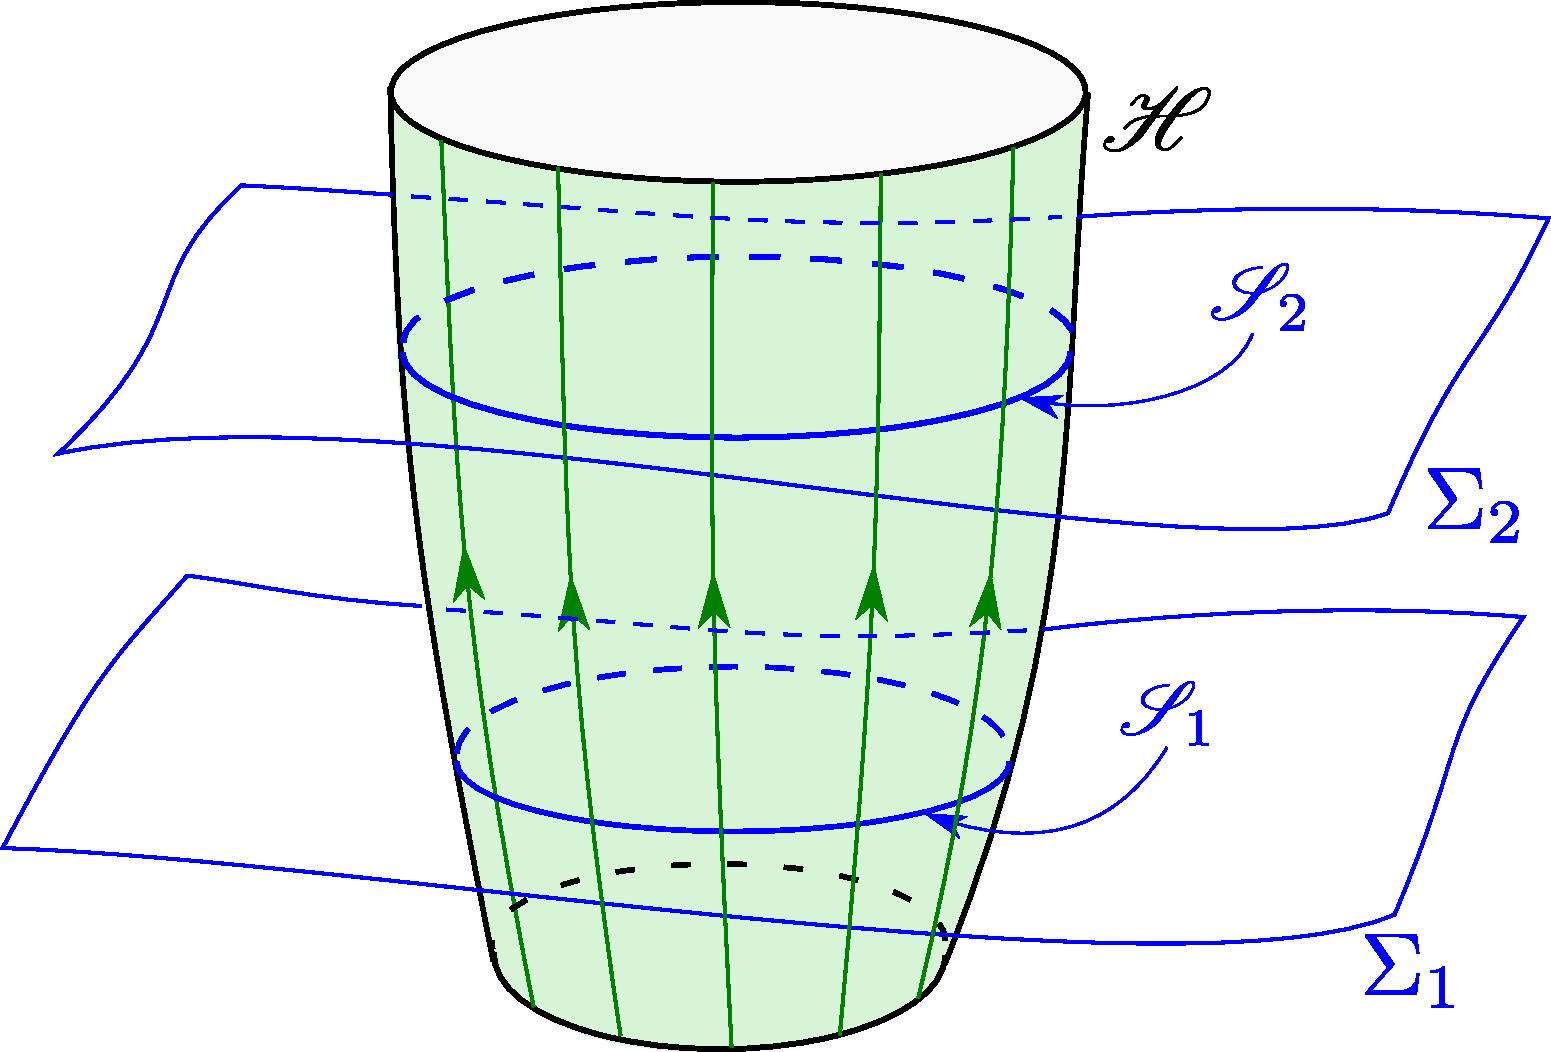
\includegraphics[width=0.6\textwidth]{evo_area_thm_smooth.pdf}}
\caption[]{\label{f:evo:area_thm_smooth} \footnotesize
Cross-sections $\Sp_1$ and $\Sp_2$ induced by the spacelike hypersurfaces $\Sigma_1$
and $\Sigma_2$ in a smooth part of the event horizon $\Hor$,
such that $\Sp_1$ and $\Sp_2$ are intersected by the same null geodesic
generators of $\Hor$ (green curves).}
\end{figure}



\begin{prop}[area theorem\index{area!theorem} \textnormal{(Hawking\index[pers]{Hawking, S.W.} 1971 \cite{Hawki71},
Chru\'sciel\index[pers]{Chrusciel, P.T.@Chru\'sciel, P.T.},
Delay\index[pers]{Delay, E.},
Galloway\index[pers]{Galloway, G.J.} and Howard\index[pers]{Howard, R.} 2001
\cite{ChrusDGH01})}]
\label{p:evo:area_thm}
Let $(\M,\w{g})$ be a $n$-dimensional spacetime containing a black hole
of event horizon $\Hor$ and such that the Ricci tensor $\w{R}$ fulfills the null
convergence condition\index{null!convergence condition}\index{convergence!condition!null --} (\ref{e:neh:null_energy_cond}), i.e.
$\w{R}(\wl, \wl) \geq 0$ for any null vector $\wl$
--- which holds in general relativity if the null energy condition\index{null!energy condition}\index{energy!condition!null --} (\ref{e:neh:null_energy_cond_matter}) is fulfilled.
Let $\Sigma_1$ and $\Sigma_2$ be spacelike hypersurfaces
such that $\Sigma_2$ lies in the causal future of $\Sigma_1$: $\Sigma_2\subset J^+(\Sigma_1)$
(cf. Sec.~\ref{s:glo:causal_struct}). Let $\Sp_1 = \Hor \cap \Sigma_1$
and $\Sp_2 = \Hor\cap\Sigma_2$.
If
\begin{itemize}
\item[(i)] $\Hor$ is smooth between $\Sp_1$ and $\Sp_2$, and $\Sp_1$ and $\Sp_2$
are cross-sections\footnote{If $\Hor$ is smooth between $\Sp_1$ and $\Sp_2$,
it is necessarily a null hypersurface there (Property~\ref{p:glo:prop4} on p.~\pageref{p:glo:prop4}),
so that the concept of cross-section as defined in Sec.~\ref{s:def:spacelike_sections}
makes sense.} of $\Hor$ that are intersected by the same null geodesic generators of $\Hor$
(cf. Fig.~\ref{f:evo:area_thm_smooth})
\end{itemize}
or
\begin{itemize}
\item[(ii)]
the closure of $J^-(\scri^+)\cup \Hor$ in
the conformal manifold $\tilde{\M}\supset\M$ defining $\scri^+$
is included in a globally hyperbolic
region $\mathscr{V}$ of $(\tilde{\M},\tilde{\w{g}})$
and $\Sigma_1$ and $\Sigma_2$ are Cauchy surfaces
of $\mathscr{V}$,
\end{itemize}
then the areas $A(\Sp_1)$ and $A(\Sp_2)$ obey
\be \label{e:evo:AS2_ge_AS1}
    A(\Sp_2) \geq A(\Sp_1) .
\ee
\end{prop}

\begin{figure}
\centerline{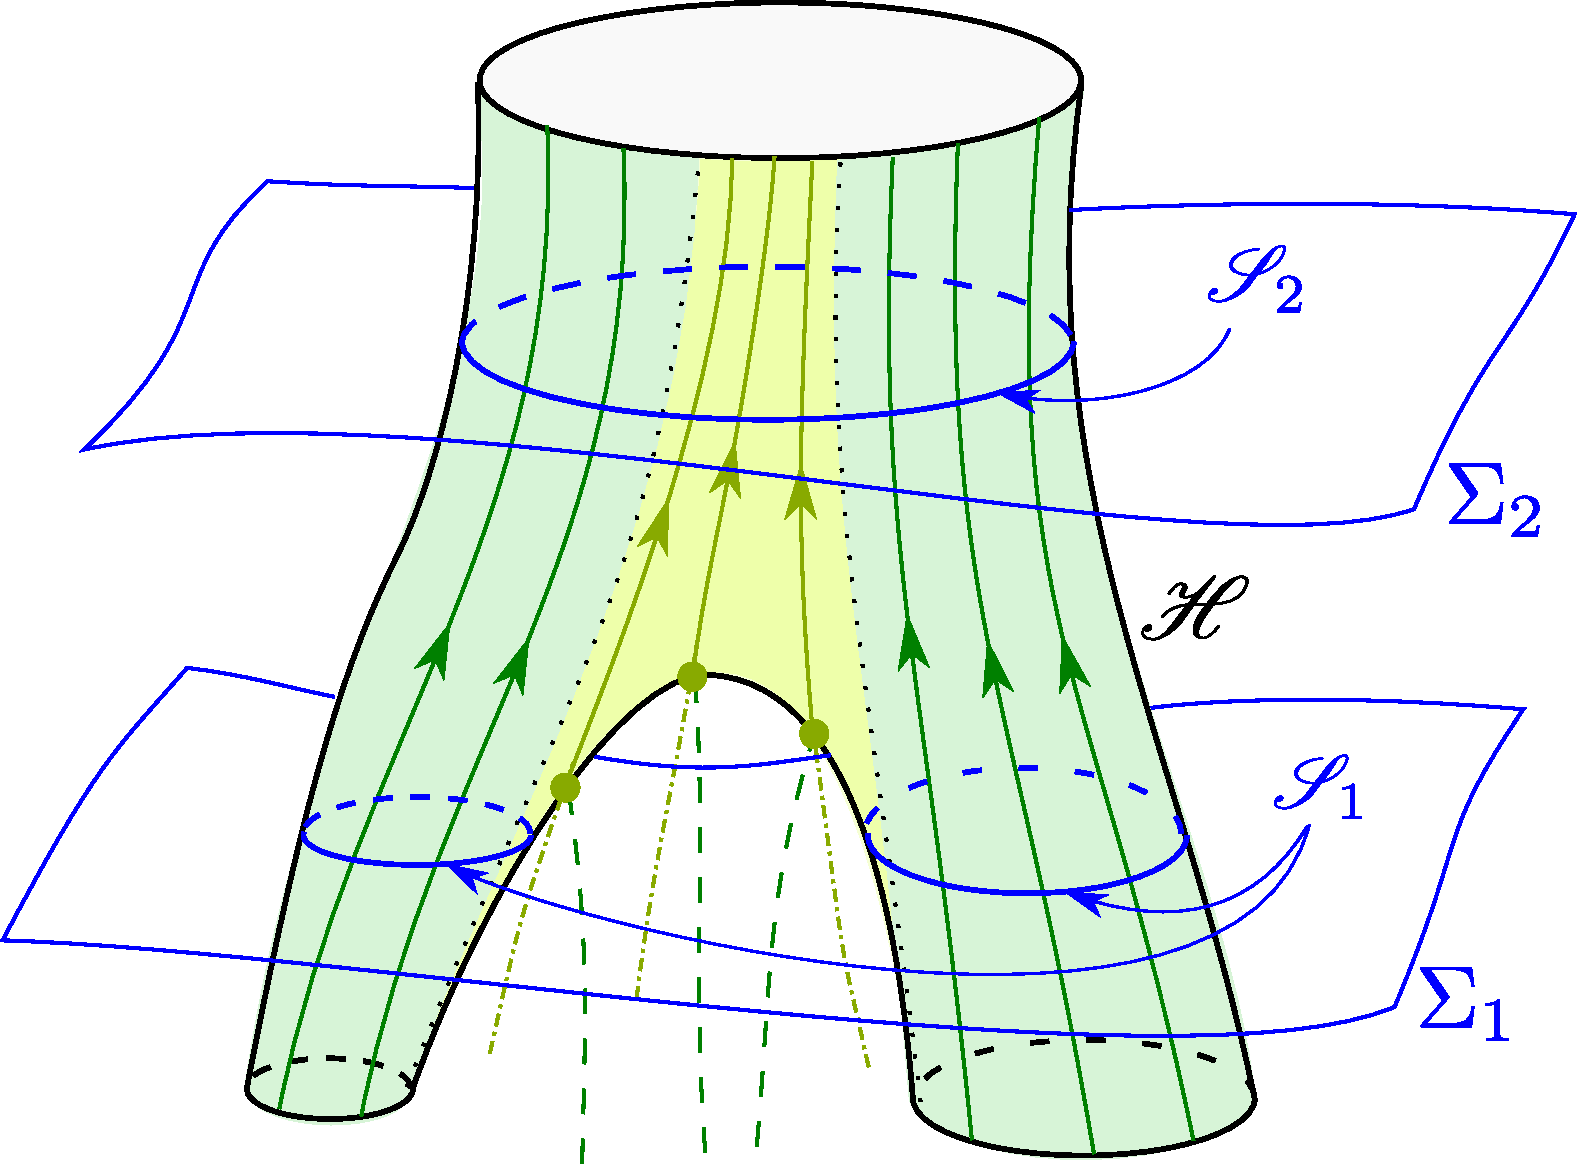
\includegraphics[width=0.6\textwidth]{evo_area_theorem.pdf}}
\caption[]{\label{f:evo:area_theorem} \footnotesize
Surfaces $\Sp_1$ and $\Sp_2$ induced by the spacelike hypersurfaces $\Sigma_1$
and $\Sigma_2$ on the event horizon $\Hor$ corresponding to a black hole merger.
All solid dark green and light green curves are null geodesic generators of $\Hor$.
The light green part of $\Hor$ is generated by null geodesics that
entered $\Hor$ at some caustic points (three of them are indicated as
light green dots); the parts of these geodesics outside $\Hor$ are drawn as
light green dot-dashed curves. The dark green dashed curves depict other null geodesics that
enter $\Hor$ at the same caustic points.}
\end{figure}


\begin{proof}
Let us consider first the case (i) ($\Hor$ smooth between
$\Sp_1$ and $\Sp_2$).
$\Sp_1$ and $\Sp_2$ are then cross-sections of $\Hor$
that are connected by null geodesic generators of $\Hor$
(cf. Fig.~\ref{f:evo:area_thm_smooth}).
One may introduce a 1-parameter foliation $(S_t)_{t\in [0,1]}$ of $\Hor$ by
cross-sections $S_t$ such that $S_0 = \Sp_1$ and $S_1 = \Sp_2$
(cf. the proof of Property~\ref{p:neh:invariance_area} for details, $\lambda$
playing the role of $t$ there). The label $t$
can then be considered as a parameter along the null geodesic generators of $\Hor$
connecting $\Sp_1$ to $\Sp_2$.
Let $\wl = \D\w{x}/\D t$ be the associated tangent vector.
Given that $\Sp_2$ lies in the future of $\Sp_1$, $\wl$ is future-directed.
By the very definition
of the expansion $\theta_{(\wl)}$ along $\wl$ [Eq.~(\ref{e:def:def_expansion})
combined with Eq.~(\ref{e:def:A_sqrt_q})], one has
\[
    \derd{}{t} A(S_t) = \int_{S_t} \theta_{(\wl)} \,  \sqrt{q} \, \D x^2 \cdots \D x^{n-1} ,
\]
where $(x^2, \ldots, x^{n-1})$ is a coordinate system on $S_t$ and $q$ is
the determinant with respect to these coordinates of the metric
induced by $\w{g}$ on $S_t$.
Now, if the null convergence condition holds, Property~\ref{p:evo:positive_expansion} implies
$\theta_{(\wl)} \geq 0$; hence
\[
  \derd{}{t} A(S_t) \geq 0 .
\]
It follows that $t\mapsto A(S_t)$ is a nondecreasing function. Consequently, $A(S_1) \geq A(S_0)$
and Eq.~(\ref{e:evo:AS2_ge_AS1}) holds.

If $\Hor$ is not smooth between $\Sp_1$ and $\Sp_2$, this is due to the crease set\index{crease set},
i.e. the subset of $\Hor$ where new null geodesics enter $\Hor$ (cf. Sec.~\ref{s:glo:properties_H}).
Naively, this reinforces the inequality $A(\Sp_2) > A(\Sp_1)$ since the new geodesics
are generating new parts of $\Hor$ and therefore parts of $\Sp_2$ distinct
from those that can be connected to $\Sp_1$ by null geodesic generators
(cf. Fig.~\ref{f:evo:area_theorem}). More precisely, let us assume (ii) and
let us consider a point $p\in\Sp_1$. Let $\Li$ be the null geodesic
generator of $\Hor$ through $p$. By property~\ref{p:glo:prop3}, $\Li$ stays in $\Hor$ for all its future after $p$. Since $\Sigma_2$ is a Cauchy surface lying in the causal future of $\Sigma_1$, $\Li$
necessarily intersects $\Sigma_2$ at a unique point $q \in \Sigma_2\cap\Hor = \Sp_2$.
Hence every point of $\Sp_1$ is mapped to a point of $\Sp_2$ by a null geodesic generator.
Let $\Sp_2^*$ be the part of $\Sp_2$ covered by this map.
If we assume that the part of $\Hor$ between $\Sp_1$ and $\Sp_2^*$ is smooth,
we may apply (i) to the pair $(\Sp_1, \Sp_2^*)$
and get $A(\Sp_2^*) \geq A(\Sp_1)$. Given that $\Sp_2^* \subset \Sp_2$, one has
$A(\Sp_2) \geq A(\Sp_2^*)$ and (\ref{e:evo:AS2_ge_AS1}) follows.
We refer to the article \cite{ChrusDGH01} for the proof in the case where
$\Hor$ is not assumed smooth between $\Sp_1$ and $\Sp_2^*$ (70 pages!).
\end{proof}

\begin{example}[Oppenheimer-Snyder collapse]
Let us consider the black hole formed by the collapse
of a ball of pressureless matter, as described by the Oppenheimer-Snyder
model studied in Sec.~\ref{s:lem:OS}. Let $\Sp_{\ti}$ be a
cross-section of the event horizon at constant ingoing Eddington-Finkelstein coordinate $\ti$.
The area of $\Sp_{\ti}$ is simply $A = 4\pi r^2$,
where $r$ is the areal radius (cf. Sec.~\ref{s:lem:OS:BH_formation}). Its
evolution can thus be read directly on Fig.~\ref{f:lem:OS:diag_int_EF} (right):
it is increasing from $A = 0$ (at $\ti\simeq 5.6\, m$) to the Schwarzschild
value $A = 16\pi m^2$ (at $\ti\simeq 9.7\, m$). This fully agrees
with the area theorem, given that the null energy condition (\ref{e:neh:null_energy_cond_matter})
is fulfilled by the energy-momentum tensor (\ref{e:lem:T_pressureless}) of the collapsing matter: $\w{T}(\wl,\wl) =  \rho (\w{u}\cdot\wl)^2 \geq 0$ since $\rho \geq 0$.
\end{example}

\begin{example}[Vaidya collapse]
Similarly, we check on Figs.~\ref{f:vai:diag_S0} and \ref{f:vai:diag_S2}
that for the radiation shell collapse studied in Chap.~\ref{s:vai},
the area of cross-sections of the event horizon
at constant ingoing Eddington-Finkelstein coordinate $t$
is increasing towards the future, for $r$ is again the areal radius
[cf. the metric (\ref{e:vai:metric_IEF})]. As we have already noticed in
Sec.~\ref{s:vai:general}, the radiation energy-momentum tensor (\ref{e:vai:ener_mom_tensor})
fulfills the null energy condition, given that $M'(v) \geq 0$ (cf. Fig.~\ref{f:vai:mass_function}).
\end{example}


\begin{hist}
It has been noticed in 1970 (published 1971) by Roger Penrose\index[pers]{Penrose, R.}
and Roger Floyd\index[pers]{Floyd, R.M.} \cite{PenroF71}
that the area of a Kerr black hole increases, despite its mass is decreasing, when
some energy is extracted by means of a Penrose process, as described in Sec.~\ref{s:gek:Penrose_proc}. Soon after, in 1971, Stephen Hawking\index[pers]{Hawking, S.W.}
\cite{Hawki71} established the area theorem for generic
dynamical black holes and a detailed proof was given in
Hawking \& Ellis' 1973 textbook (Proposition~9.2.7 in \cite{HawkiE73}).
In 2001, Piotr Chru\'sciel\index[pers]{Chrusciel, P.T.@Chru\'sciel, P.T.},
Erwann Delay\index[pers]{Delay, E.},
Gregory Galloway\index[pers]{Galloway, G.J.} and Ralph Howard\index[pers]{Howard, R.}
\cite{ChrusDGH01} pointed out that the Hawking \& Ellis proof is
valid only for $\Hor$ piecewise smooth (cf. the
discussion in Sec.~3.5.1 of Chru\'sciel's textbook \cite{Chrus20}); they constructed
a new proof that does not assume the smoothness of $\Hor$.
\end{hist}

\subsection{A second law?}

Basically the area theorem~\ref{p:evo:area_thm} states that
the area of cross-sections of a black hole event horizon
cannot decrease from the past to the future.
By its irreversible character, this property bears some resemblance
with the second law of thermodynamics.
By itself, this is of course not sufficient to identify the black hole area
with some entropy (any nondecaying physical quantity has not to be an entropy!).
However, we have seen in Sec.~\ref{s:evo:a_first_law_question} that the
candidate $T\D S$ term for a possible first law could be $\kappa/(8\pi)\D A$.
It is thus tempting to identify $A$ with an entropy $S$, up to some
constant factor $\alpha$. Then the temperature $T$ would be $\kappa/(8\pi\alpha)$:
\begin{subequations}
\label{e:evo:identif_S_T}
\begin{align}
  S & = \alpha A \label{e:evo:identif_S_A}\\
  T &= \frac{1}{8 \pi\alpha}\, \kappa , \label{e:evo:identif_T_kappa}
\end{align}
\end{subequations}
so that we get $T\D S = \kappa/(8\pi)\D A$, making
the mass variation formula (\ref{e:evo:mass_variation_vacuum_n4}) look pretty much like
the first law of thermodynamics.

%%%%%%%%%%%%%%%%%%%%%%%%%%%%%%%%%%%%%%%%%%%%%%%%%%%%%%%%%%%%%%%%%%%%%%%%%%%%%%%

\section{The other laws of black hole dynamics}

\subsection{Zeroth law}

We have already established a so-called \emph{zeroth law of black hole dynamics}
in Chap.~\ref{s:neh}, namely the surface gravity
$\kappa$ of a Killing horizon is constant, provided that the
null dominance condition is fulfilled (Property~\ref{p:neh:zeroth_law})
or that the Killing horizon is part of a bifurcate Killing horizon
(Property~\ref{p:neh:zeroth_law_bifur}).
Now, by Properties~\ref{p:sta:H_Killing_hor_xi_null}
and \ref{p:sta:strong_rigidity_thm}, (a connected component of) the event horizon
of a stationary black hole must be a Killing horizon. Hence, we may extend
the zeroth law to black holes\index{zeroth law!of BH dynamics}:

\begin{prop}[zeroth law of black hole dynamics]
\label{p:evo:zeroth_law}
Let $(\M,\w{g})$ be a stationary spacetime of dimension $n\geq 4$
containing a black hole.
Let $\Hor$ be a connected component of the black hole event horizon.
If $\Hor$ is non-rotating (i.e. if the stationary Killing vector $\w{\xi}$ is null
on $\Hor$), $\Hor$ is necessarily a Killing horizon (Property~\ref{p:sta:H_Killing_hor_xi_null}).
If $\Hor$ is rotating
($\w{\xi}$ spacelike on some parts of $\Hor$),
we shall assume that the hypotheses of the strong rigidity theorem
(Property~\ref{p:sta:strong_rigidity_thm}) hold, so that $\Hor$ is a Killing horizon as well.
If the null dominance condition\index{null!dominance condition}\index{dominance!null -- condition} (\ref{e:neh:null_dominant_cond})
is fulfilled on $\Hor$  --- which is guaranteed in general relativity
if the null dominant energy condition\index{null!dominant energy condition}\index{energy!condition!null dominant --} (\ref{e:neh:null_dominant_cond_T}) holds on $\Hor$ ---
or if $\Hor$ is part of a bifurcate Killing horizon,
then the surface gravity $\kappa$ is constant over $\Hor$.
\end{prop}

Given that a black hole ``in equilibrium'' is modeled by a black hole in
a stationary spacetime,
this property bears a strong resemblance with
the \emph{zeroth law of thermodynamics}\index{zeroth law!of thermodynamics}, which states that the temperature of a body in equilibrium
is uniform over the entire body.
This strengthens the interpretation of the surface gravity
$\kappa$ as the temperature $T$ (up to some factor) performed in
Eq.~(\ref{e:evo:identif_S_T}).


\subsection{What about the third law?}

The classical Nernst formulation of the \emph{third law of thermodynamics}\index{third law!of thermodynamics}
states that the entropy of a system must approach zero (or a universal constant)
as its temperature tends to zero. In this form and with the identification (\ref{e:evo:identif_S_T}), this law certainly does not hold for black holes, because
extremal black holes, which have $\kappa=0$, have a non-vanishing area. For
instance, the area of the extremal Kerr black hole\index{extremal!Kerr spacetime}\index{Kerr!extremal -- spacetime} of mass $m$ (Chap.~\ref{s:exk}) is
$A = 8\pi m^2$ (take the limit $a\to m$ in Eq.~(\ref{e:ker:A_a_m})),
which is neither zero, nor a universal constant. Similarly, the area of
the extremal Reissner-Nordström black hole\index{Reissner-Nordström!black hole!extremal --}\index{extremal!Reissner-Nordström!black hole} of mass $m$ is $A = 4\pi m^2$
(this is immediate from the metric (\ref{e:loc:metric_ERN}) below).
Another formulation of the third law of thermodynamics states that it is impossible to bring any
system to zero temperature by a finite number of operations. This was the formulation adopted
for black holes, as a conjecture, in 1973 by Carter\index[pers]{Carter, B.} \cite{Carte73b} and Bardeen\index[pers]{Bardeen, J.M.}, Carter and Hawking\index[pers]{Hawking, S.W.} \cite{BardeCH73}.
It was then reformulated, with a tentative proof, by Israel\index[pers]{Israel, W.} in 1986 \cite{Israe86b}, as
\begin{quote}
No continuous process in which the energy-momentum tensor of accreted matter remains
bounded and satisfies the weak energy
condition\index{weak!energy condition}\index{energy!condition!weak --} in a neighborhood of the apparent
horizon can reduce the surface gravity of a black hole to zero
within a finite advanced time.
\end{quote}
However, as pointed out recently by Kehle\index[pers]{Kehle, C.} and Unger\index[pers]{Unger, R.} \cite{KehleU23}, Israel's proof
is restricted to the case where outermost trapped surfaces evolve smoothly, while, as we shall discuss in Chap.~\ref{s:loc},
their evolution generically presents discontinuous jumps, even if the spacetime
and all the matter fields remain perfectly smooth. In particular, Kehle and Unger \cite{KehleU23} have exhibited
a spacetime where the collapse of a $C^k$-regular charged scalar field (obeying the dominant, and hence the weak, energy condition) turns a (piece of) Schwarzschild black hole
into an extremal Reissner-Nordström black hole within a finite advanced time\footnote{As shown
in Sec.~5.5.6 of Poisson's textbook \cite{Poiss04}, this cannot happen with a charged null dust
(i.e. a charged generalization of Vaidya collapse discussed in Chap.~\ref{s:vai}) that obeys
the weak energy condition.}.

From an astrophysical point of view, Bardeen\index[pers]{Bardeen, J.M.} has shown in 1970 \cite{Barde70a}
that a Schwarzschild black hole
of mass $m_0$ ($\kappa = 1/(4m_0) > 0$, Eq.~(\ref{e:def:kappa_Schw_hor}))
can in principle be spun up to an extremal Kerr black hole
($\kappa = 0$)
by accreting matter from the
innermost stable circular orbit\index{innermost!stable circular orbit}\index{circular!orbit!innermost stable --}
(ISCO, cf. Sec.~\ref{s:gek:circ_orb_stab}) by a total rest-mass amount of
$\simeq 1.86\, m_0$; the mass of the final black hole is then $m \simeq 2.45\, m_0$.
However, if one assumes that the matter comes from an accretion disk\index{accretion!disk}
terminating at the ISCO and
one takes into account the electromagnetic emission of the disk, the extremal Kerr state
cannot be achieved. The reason is that a substantial part of the emitted photons carry a negative angular momentum $\ell$ and
the black hole absorption cross-section for photons with $\ell<0$ is larger than for those with
$\ell>0$. This appears clearly on the shadow picture of Fig.~\ref{f:gik:shadow_a95},
where the part $\alpha>0$, which is due to photons
with $\ell < 0$ (cf. Eq.~\ref{e:gik:shadow_param_eq_alpha}), is much larger than the part $\alpha<0$
corresponding to $\ell > 0$. Consequently, the black hole absorbs more photons with $\ell < 0$
than with $\ell>0$; this diminishes the increase of the black hole spin $a$ resulting form the accretion of  matter from the disk (which has a positive angular momentum). Thorne\index[pers]{Thorne, K.S.} has shown in 1974 \cite{Thorn74} that the balance between the two processes leads to a final spin parameter $a \simeq 0.998 \, m$, quite insensitive to the details
of the emission mechanism in the accretion disk. This is close to, but strictly lower than, the critical
value $a = m$ that would have yield a zero surface gravity. Hence, in this respect, we can say that
astrophysical black holes absorbing matter from an accretion disk obey a kind of third law of thermodynamics.
But this does not appear to arise from some fundamental properties of black holes; it rather results from the properties of their environment.

It must be stressed that in the field of standard thermodynamics as well, the third law has not the same fundamental status as the other laws.
In particular it can be violated by some rather simple systems (see Ref.~\cite{Wald97} for a discussion and an example involving a boson (or fermion) gas confined to a circular ring).

For all the above reasons, we shall no longer discuss the third law here.

%%%%%%%%%%%%%%%%%%%%%%%%%%%%%%%%%%%%%%%%%%%%%%%%%%%%%%%%%%%%%%%%%%%%%%%%%%%%%%%

\section{Black hole thermodynamics}

\subsection{The three laws}

Let us summarize the results obtained so far, in the form of three laws
analogous to the laws of thermodynamics. To stress the analogy, we are using the phrase
\emph{black hole in equilibrium}\index{black!hole!in equilibrium} for \emph{black hole in a stationary spacetime}. Besides, for the sake of brevity, we shall not repeat
the various assumptions underlying these laws, referring to previously
stated properties for all the details. Furthermore, we consider
a connected event horizon for simplicity.

\begin{prop}[laws of black hole dynamics]
\label{p:evo:laws_BH_dyn}
\begin{description}
\item[Zeroth law:] Under the hypotheses of Property~\ref{p:evo:zeroth_law},
the surface gravity $\kappa$ of the event horizon of a black hole in equilibrium is
uniform over the horizon:
\be
    \kappa = \mathrm{const}.
\ee
\item[First law:] Under the hypotheses of Property~\ref{p:evo:mass_var_electrovac},
the change $\delta M$ in total mass  between two nearby electrovacuum configurations of
a black hole in equilibrium is related to the change $\delta A$ in horizon area,
the change $\delta J$ in total angular momentum and the change
$\delta Q_{\Hor}$ in electric charge
by\footnote{For simplicity, we are considering
black holes with a connected horizon and a single angular momentum; see
Eq.~(\ref{e:evo:mass_variation_electovac}) for the general formula, where $M$ is denoted by
$M_\infty$ and $J$ by $J_\infty$.}
\be \label{e:evo:first_law}
\delta M = \frac{\kappa}{8\pi} \, \delta A + \Omega_{\Hor} \, \delta J
    + \Phi_{\Hor} \, \delta Q_{\Hor} ,
\ee
where $\Omega_{\Hor}$ and $\Phi_{\Hor}$ are the horizon's angular velocity and
electric potential respectively.
\item[Second law:] Under the hypotheses of Property~\ref{p:evo:area_thm},
the area of cross-sections of a black hole cannot decrease in time:
\be
    A(\Sp_2) \geq A(\Sp_1) ,
\ee
as soon as the cross-section $\Sp_2$ lies in the causal future of the
cross-section $\Sp_1$.
\end{description}
\end{prop}


\subsection{Hawking radiation}

From a pure classical (i.e. non-quantum) point of view, if one would like to attribute some
temperature $T$ to a black hole, it should be $T=0$, since a black hole does not radiate at all.
For a stationary black hole with nonzero surface gravity $\kappa$, this contradicts the tentative identification (\ref{e:evo:identif_S_T}) between $T$ and $\kappa$.
It is remarkable that quantum field theory in curved spacetime
restores the identification:

\begin{prop}[Hawking radiation]
Let $(\M,\w{g})$ be a $n$-dimensional ($n\geq 2$) asymptotically flat
spacetime that is stationary and contains a black hole, the event horizon
of which is a Killing horizon of constant surface gravity $\kappa$.
Then, quantum field theory in the curved background $(\M,\w{g})$
predicts that any quantum field gives birth to a thermal radiation
from the black hole to infinity, called
\defin{Hawking radiation}\index{Hawking!radiation}. The radiation temperature
as measured by asymptotic inertial observers at rest with respect to the black hole
is
\be \label{e:evo:Hawking_temp}
    \encadre{T_{\rm H} = \frac{\hbar}{k_{\rm B}} \frac{\kappa}{2\pi} } ,
\ee
where $\hbar = 1.054571817\; 10^{-34} {\rm\; J\, s}$ is the reduced Planck constant and
$k_{\rm B} = 1.380649\; 10^{-23}$ ${\rm\;  J\, K}^{-1}$ is the Boltzmann constant. $T_{\rm H}$ is called the
\defin{Hawking temperature}\index{Hawking!temperature} of the black hole.
\end{prop}

We shall not establish this property here; this is done in many textbooks,
e.g. \cite{Wald84,Wald94,FroloN98,Carro04,FabbrN05}, as well in some review
articles, e.g. \cite{BroutMPS95,Damou04}. Rather, we shall limit
ourselves to a few remarks:

\begin{remark}\label{r:evo:Hawking_temp_units}
Formula~(\ref{e:evo:Hawking_temp}) is given for $c=1$
units, which are used throughout the text. If one restores $c$ and considers
that $\kappa$ has the dimension of an acceleration, the formula should read
$T_{\rm H} = \frac{\hbar}{k_{\rm B}} \frac{\kappa}{2\pi c}$.
\end{remark}

\begin{remark}
The phenomenon of Hawking radiation is essentially kinematic and does not depend on any field equation for the
metric $\w{g}$. In particular it does not rely on the Einstein equation.
Moreover, the Hawking temperature (\ref{e:evo:Hawking_temp}) is independent from the spacetime dimension
$n$ (see e.g. Ref.~\cite{KantiW15} for a detailed discussion).
\end{remark}

\begin{remark}\label{r:evo:local_Hawking_rad}
The Hawking temperature $T_{\rm H}$ is the radiation temperature measured
infinitely far from the black hole; it is therefore not a ``local'' temperature
at the level of the event horizon $\Hor$.
More precisely, let us assume for simplicity that the black hole is non-rotating,
(cf. Property~\ref{p:sta:xi_tangent_H}) and that its exterior is strictly static. In other words,
the stationary Killing vector $\w{\xi}$ is assumed to be null on $\Hor$  and
timelike in the black hole exterior. Let us then consider static observers at a finite distance
from $\Hor$, i.e. observers
of 4-velocity $\w{u} = \w{\xi} / V$, where $V := \sqrt{-\w{\xi}\cdot\w{\xi}}$
[cf. Eqs.~(\ref{e:neh:def_u_stationary_obs}) and (\ref{e:neh:def_V_norm_xi})].
Then these observers find the temperature of the Hawking radiation to
be\footnote{We may say
that Hawking radiation obeys \defin{Tolman-Ehrenfest law}\index{Tolman-Ehrenfest law}, which
states that the temperature $T$ of a medium in thermal equilibrium in a stationary gravitational field
obeys $T V = \mathrm{const}$ \cite{SantiV19}.}
\be \label{e:evo:Hawking_temp_local}
    T = \frac{T_{\rm H}}{V} .
\ee
For infinitely distant observers, $V\to 1$ [cf. Eq.~(\ref{e:sta:xi_scri})], and we recover $T=T_{\rm H}$.
For static observers infinitely close to the event horizon ($V\to 0$), we get
$T\to +\infty$. Note that those observers are
also experiencing a diverging acceleration [cf. Eq.~(\ref{e:neh_diverging_accel})].
On the contrary, a freely-falling observer crossing the horizon measures
$T=0$, i.e. she does not detect the Hawking radiation.
\end{remark}

\begin{remark}
The Hawking radiation is closely related to the
\defin{Unruh effect}\index{Unruh effect}, which is another prediction of quantum field theory:
in vacuum Minkowski spacetime, a uniformly accelerated observer measures a black-body radiation
of all particle species at the temperature $T_{\rm U} = (\hbar/k_{\rm B}) \, a / (2\pi)$, where
$a = \sqrt{\w{a}\cdot\w{a}}$ is the norm of the observer's 4-acceleration \cite{Unruh76,Wald94,Carro04}.
A static observer $\Obs$ close to the black hole horizon $\Hor$, as considered in Remark~\ref{r:evo:local_Hawking_rad},
feels an acceleration given by Eq.~(\ref{e:neh:kappa_lim_Va}): $a \sim \kappa / V$.
By combining formulas~(\ref{e:evo:Hawking_temp_local}) and (\ref{e:evo:Hawking_temp}),
we may then rewrite the radiation temperature $T$ measured by $\Obs$ as
$T \sim (\hbar/k_{\rm B}) \, a / (2\pi)$. Hence, it coincides with the Unruh temperature $T_{\rm U}$ of
the observer in Minkowski spacetime sharing the same acceleration $a$ as $\Obs$, which is somehow expected
if one assumes that freely-falling observers near $\Hor$ perceive quantum states identical to
the Minkowski vacuum (no radiation).
\end{remark}

\begin{remark} \label{r:evo:comp_Hawking_rad}
In terms of elementary particles, the Hawking radiation is composed of
all existing species of massless and massive particles. For the latter ones,
the contribution is significant only if
$k_{\rm B} T_{\rm H} > m_{\rm p}$, where $m_{\rm p}$ is the particle's mass.
For Schwarzschild black holes of mass $M \gg 2\; 10^{13} {\rm\; kg}$ (the threshold
for $k_{\rm B} T_{\rm H}$ being equal to the electron mass, see below), the Hawking radiation
is composed quasi-exclusively of neutrinos ($87\%$ of the radiated energy),
photons ($12\%$) and possibly gravitons ($1\%$) \cite{Page76,ThornZP86}.
\end{remark}

\begin{remark}
The observed radiation spectrum at infinity is not exactly that
of a black body\index{black!body} of temperature $T_{\rm H}$: it is corrected
by greybody factors, which take into account the interaction of the radiation
with the spacetime curvature (backscattering).
\end{remark}

For a Kerr black hole, the surface gravity is given by formula (\ref{e:ker:kappa_m_a}),
so that the Hawking temperature can be expressed in terms
of the black hole mass $M=m$ and the dimensionless spin parameter
$\bar{a} := a/m = J/M^2$ ($0\leq \bar{a}\leq 1$):
\be \label{e:evo:T_H_Kerr}
   \encadre{ T_{\rm H} = \frac{\hbar}{k_{\rm B}} \frac{c^3}{8\pi G M}
   \; \frac{2}{1 + (1 - \bar{a}^2)^{-1/2}} } _{\rm\; Kerr}.
\ee
Note that we have restored the gravitational constant $G$ and the speed of light $c$
(cf. Remark~\ref{r:evo:Hawking_temp_units}). Numerically, we get
\be
    T_{\rm H} = 6.17\; 10^{-8} \left( \frac{M_\odot}{M} \right)
    \frac{2}{1 + (1 - \bar{a}^2)^{-1/2}} {\rm\; K},
\ee
or, in units more adapted to small black holes,
\be
    k_{\rm B} T_{\rm H}= 1.057\; 10^{10} \left( \frac{1 {\rm\; kg}}{M} \right)
    \frac{2}{1 + (1 - \bar{a}^2)^{-1/2}} {\rm\; GeV}.
\ee
Hence, for a Schwarzschild black hole ($\bar{a}=0$),
$T_{\rm H} = 6.17\; 10^{-8} ({M_\odot}/{M}) {\rm\; K}$. For astrophysical black holes,
this leads to tiny temperatures: $T_{\rm H} \simeq 4\; 10^{-9} {\rm\; K}$
for a $15 \, M_\odot$ stellar black hole (e.g. Cyg X-1, cf. Table~\ref{t:ges:time_free_fall}),
$T_{\rm H} \simeq 1.6\; 10^{-14} {\rm\; K}$ for the Milky Way central black hole Sgr~A*
($M=4.1\; 10^{6} \, M_\odot$)
and $T_{\rm H} \simeq 9\; 10^{-18} {\rm\; K}$ for M87*
($M=6.5\; 10^{9} \, M_\odot$). The value $T_{\rm H} = 1 {\rm\; K}$ is achieved
for a black hole of mass $6.17\; 10^{-8} \, M_\odot$, i.e. $2\, \%$ of the
Earth's mass, while the value $k_{\rm B} T_{\rm H} = m_{\rm e} c^2$
($m_{\rm e} = 9.11\; 10^{-31}\; {\rm kg}$ being the electron mass) is achieved
for $M = 2.07\; 10^{13}\; {\rm kg}$.

Another conclusion that one can draw from formula (\ref{e:evo:T_H_Kerr}) is
that $T_{\rm H}=0$ for an extremal Kerr black hole\index{extremal!Kerr!spacetime}\index{Kerr!extremal -- spacetime} ($\bar{a}=1$): such an object does not emit any Hawking radiation.

Since it emits some radiation to infinity, the black hole loses energy, which
makes its mass decrease. For a Kerr black hole, according to formula~(\ref{e:evo:T_H_Kerr}),
this yields a temperature increase and hence an enhanced Hawking radiation. Furthermore,
the higher the temperature,
the more quantum fields can join the radiation
(cf. Remark~\ref{r:evo:comp_Hawking_rad}), which enhances
the rate of energy loss as well. We are thus facing a runaway process, in which the whole
black hole eventually disappears --- a phenomenon called
\defin{Hawking evaporation}\index{Hawking!evaporation} or
\defin{black hole evaporation}\index{black!hole!evaporation}\index{evaporation (black hole)}.
However, this evaporation occurs on extremely long time scales for astrophysical black holes.
To get a rough estimate of the evaporation time, let us consider
that the total power
(energy radiated per unit time or luminosity) $L$ of Hawking radiation received at infinity
obeys the Stefan-Boltzmann law\index{Stefan-Boltzmann law}:
$L = \mathcal{A} \sigma T_{\rm H}^4$, where $\sigma$ is Stefan-Boltzmann constant:
$\sigma = \pi^2 k_{\rm B}^4/(60 \hbar^3)$ and $\mathcal{A}$ is some ``emission area''.
For simplicity, let us restrict to a Schwarzschild black hole of mass $M$. Then, a value
of $\mathcal{A}$ suitable to get some estimate is
$\mathcal{A} = 4\pi b_{\rm c}^2$, where
$b_{\rm c} = 3\sqrt{3} M$ is the critical impact parameter for null geodesics
introduced in Chap.~\ref{s:gis} [cf. Eq.~(\ref{e:ges:b_crit})]. Indeed, $4 \pi b_{\rm c}^2$
can be viewed as the black hole's area ``seen from infinity'' (cf. Fig.~\ref{f:gis:shadow}).
Moreover, it can be shown that the spectrum of Hawking radiation at high frequencies (i.e. $\nu \gg M^{-1}$, so that the quantum fields can be treated within geometrical optics) is that of a black
body of temperature $T_{\rm H}$ and total area $4\pi \times 27 M^2$ (see Fig.~1 of Ref.~\cite{Page76}). Hence
$\mathcal{A} = 108\pi M^2$. Given that
$k_{\rm B} T_{\rm H} = \hbar/(8\pi M)$ [Eq.~(\ref{e:evo:T_H_Kerr}) with $\bar{a}=0$],
Stefan-Boltzmann law yields
\be \label{e:evo:Hawking_rad_power}
    L = C \frac{\hbar}{M^2} ,
\ee
where $C = 9 / (20480\pi) \simeq 1.40\; 10^{-4}$ is a dimensionless constant.
Acually, a precise computation, taking
into account the propagation of quantum fields in the Schwarzschild geometry
and various particle species
leads to the same formula (\ref{e:evo:Hawking_rad_power}) with \cite{ThornZP86,Page76,Page05}
\be \label{e:evo:Hawking_rad_power_alpha}
    C = 2.83\; 10^{-4}.
\ee
This value is valid for $M \gg 2\; 10^{13} {\rm\; kg}$ ($T_{\rm H}$
below the electron threshold, cf. Remark~\ref{r:evo:comp_Hawking_rad}), so that the Hawking radiation
contains only photons, neutrinos and gravitons\footnote{The original computation,
performed by Page\index[pers]{Page, D.N.} in 1976 \cite{Page76}, resulted
in $C=2.01\; 10^{-4}$ but it took into account only the four species
of neutrinos known at that time ($\nu_{\rm e}$, $\bar{\nu}_{\rm e}$, $\nu_\mu$ and
$\bar{\nu}_\mu$), in addition to photons and gravitons. It has been updated
by adding the tau neutrinos ($\nu_\tau$ and $\bar{\nu}_\tau$)
by Thorne, Zurek \& Price in 1986 \cite{ThornZP86}.
The value (\ref{e:evo:Hawking_rad_power_alpha}) is also recovered by
setting $n_{1/2}=3$, $n_1=1$ and $n_2=1$ in Eq.~(19) of Page's review article~\cite{Page05}.}.
The black hole mass decreases according to $\D M/\D t = - L$, i.e.
\be \label{e:evo:Hawking_rad_mass_decrease}
    \derd{M}{t} = - C \frac{\hbar}{M^2} .
\ee
Here $t$ is the time measured by an inertial observer at infinity.
This differential equation is easily integrated into
\be
    M(t) = \left( M_0^3 - 3 C \hbar t \right) ^{1/3} ,
\ee
where $M_0$ is the mass at $t=0$. Defining the evaporation time $t_{\rm evap}$
as the time to reach $M=0$ from $M = M_0$, we get immediately
\be \label{e:evo:t_evap}
    t_{\rm evap} = \frac{M_0^3}{3C\hbar} .
\ee
With $C$ given by
(\ref{e:evo:Hawking_rad_power_alpha}), this yields the numerical value
\be
    t_{\rm evap} = 1.54\; 10^{66} \left( \frac{M_0}{M_\odot} \right) ^3 {\rm\; yr} .
\ee
For an astrophysical black hole ($M_0 >  1 M_\odot$), this is a huge duration --- more than 56
orders of magnitude larger than the Universe's age ($t_{\rm Univ} \simeq 1.38\; 10^{10} {\rm\; yr}$)!
We conclude that for astrophysical black holes, the Hawking radiation is ultra-negligible and
does not play any role in the black hole dynamics. Hawking radiation becomes relevant only when
$t_{\rm evap} < t_{\rm Univ}$, say. From Eq.~(\ref{e:evo:t_evap}), we get
$t_{\rm evap} < t_{\rm Univ} \iff M_0 < 4.15\; 10^{11} {\rm\; kg}$. Actually, this value
is below $2\; 10^{13}{\rm\; kg}$ so that electrons, and even muons, should have been included into the Hawking radiation
(cf. Remark~\ref{r:evo:comp_Hawking_rad}). However, the above estimate is pretty good, a precise computation leading to \cite{MacGiCP08}
\be
    t_{\rm evap} < t_{\rm Univ} \iff M_0 < 5.00\; 10^{11} {\rm\; kg} .
\ee
The upper bound is roughly the mass of an asteroid of half-kilometer size.
Note that a black hole of that mass has a Schwarzschild radius
of only $0.74{\rm \; fm}$ (around the proton size!); it
would pertain to the hypothetical class
of the so-called
\defin{primordial black holes}\index{primordial black hole}\index{black!hole!primordial --},
i.e. black holes of subsolar mass that could have been formed in the primordial universe
(see e.g. \cite{CarrKSY21} for a review).

\begin{remark}
For a Schwarzschild-like black hole, the horizon area $A$ is proportional to the square
of the mass: $A = 16\pi M^2$ [Eq.~(\ref{e:neh:area_Schwarz})], so that
the evolution law~(\ref{e:evo:Hawking_rad_mass_decrease}) implies $\D A / \D t < 0$.
In other words, the horizon area decreases as the black hole evaporates via Hawking radiation.
At frst glance,  this seems to contradict the second law of black hole dynamics
(Property~\ref{p:evo:laws_BH_dyn}), i.e. the
area theorem~\ref{p:evo:area_thm}.
Actually there is no contradiction since one of the hypotheses of
the area theorem is not fulfilled for evaporating black holes, namely
the null convergence condition. Indeed, the effective energy-momentum tensor\footnote{See e.g.
Ref.~\cite{FroloT89} for the computation of the renormalized expectation value of the energy-momentum tensor of a quantum field near the black hole horizon.}
of the quantum fields generating the Hawking radiation does not obey the
null energy condition (\ref{e:neh:null_energy_cond_matter}).
\end{remark}

\subsection{Bekenstein-Hawking entropy}

The phenomenon of Hawking radiation puts on firm grounds the identification
of the surface gravity as the black hole temperature and fully fixes the coefficient $\alpha$
appearing in Eq.~(\ref{e:evo:identif_S_T}): comparing Eq.~(\ref{e:evo:identif_T_kappa})
with formula~(\ref{e:evo:Hawking_temp}) for $T=T_{\rm H}$, we get $\alpha = k_{\rm B}/(4\hbar)$. Accordingly, Eq.~(\ref{e:evo:identif_S_A}) becomes
$S = k_{\rm B} A/(4\hbar)$ and we may state
\begin{prop}[Bekenstein-Hawking entropy]
A black hole in equilibrium
is endowed with the \defin{Bekenstein-Hawking entropy}\index{Bekenstein-Hawking entropy}\index{entropy!Bekenstein-Hawking --} $S_{\rm BH}$, which is proportional to the black hole area $A$ according to the formula:
\be \label{e:evo:S_BH}
    \encadre{S_{\rm BH} = k_{\rm B}\frac{A}{4\hbar} }.
\ee
The first law of black hole dynamics (\ref{e:evo:first_law}) writes then
\be
    \delta M = T_{\rm H} \, \delta S_{\rm BH} + \Omega_{\Hor} \, \delta J
    + \Phi_{\Hor} \, \delta Q_{\Hor} ,
\ee
where $T_{\rm H}$ is the Hawking temperature.
\end{prop}

\begin{remark}
If one restores the $G$'s and $c$'s, formula~(\ref{e:evo:S_BH}) reads
$S_{\rm BH} = k_{\rm B}\frac{c^3 A}{4G \hbar}$. One then recognizes the square
of the \defin{Planck length}\index{Planck!length}:
$\ell_{\rm P} := \sqrt{G\hbar / c^3} \simeq 1.62\; 10^{-35} {\rm\; m}$,
so that formula~(\ref{e:evo:S_BH}) can be rewritten in terms of the
dimensionless ratio $A/\ell_{\rm P}^2$ as
\be
    S_{\rm BH} = k_{\rm B}\frac{A}{4\ell_{\rm P}^2} .
\ee
\end{remark}

For a Kerr black hole, the area $A$ is related to the mass $M$ and to the spin
parameter $a = \bar{a} M$ via Eq.~(\ref{e:ker:A_a_m}),
so that the Bekenstein-Hawking entropy (\ref{e:evo:S_BH}) can be expressed as
\be
    \encadre{S_{\rm BH} = 4\pi k_{\rm B} \frac{G M^2}{\hbar c} \,
        \frac{1 + \sqrt{1 - \bar{a}^2}}{2} } _{\rm\; Kerr} .
\ee
Note that, as in formula~(\ref{e:evo:T_H_Kerr}) for the Hawking temperature,
we have restored $G$ and $c$ in the above formula. Numerically, we get
\be
    S_{\rm BH} = 1.05\; 10^{77}\; \left( \frac{M}{M_\odot} \right) ^2
    \frac{1 + \sqrt{1 - \bar{a}^2}}{2} \; k_{\rm B} .
\ee
Hence, for a Schwarzschild black hole ($\bar{a} = 0$),
$S_{\rm BH} = 1.05\; 10^{77} (M/M_\odot)^2  \; k_{\rm B}$.
This yields huge values for astrophysical black holes:
$S_{\rm BH} \simeq 2\; 10^{79} \, k_{\rm B}$
for a $15 \, M_\odot$ stellar black hole,
$S_{\rm BH} \simeq 2\; 10^{90} \, k_{\rm B}$ for Sgr~A*
($M=4.1\; 10^{6} \, M_\odot$)
and $S_{\rm BH} \simeq 4\; 10^{96} \, k_{\rm B}$
for M87* ($M=6.5\; 10^{9} \, M_\odot$).
These numbers are terribly large: besides black holes, the total entropy of the observable
Universe is about $1.1\; 10^{90} \, k_{\rm B}$, mostly from the
cosmic microwave background\index{cosmic!microwave background}
and the cosmic neutrino background\index{cosmic!neutrino background}
(roughly one half each), largely
dominating the entropy of the interstellar and galactic medium ($\sim 10^{82}\, k_{\rm B}$)
and that of all the stars ($\sim  10^{81}  \, k_{\rm B}$) \cite{EganL10}.
In particular, the entropy of a single massive black hole, such as Sgr~A* or M~87*,
is larger than the entropy of the whole observable Universe!



\subsection{The generalized second law}


